% Main template for University of Bayreuth thesis
\documentclass[12pt,a4paper]{report}

% Import custom packages and settings


% Set page geometry
\usepackage[a4paper,margin=2.5cm]{geometry}
\usepackage{graphicx}
\usepackage{booktabs}
\usepackage{bookmark}
\usepackage{hyperref}
\usepackage[backend=biber]{biblatex}
\addbibresource{ref/MAref.bib}



% Define custom commands for metadata
\newcommand{\subtitle}{}
\newcommand{\supervisorname}{Supervisor Name}
\newcommand{\fieldofstudy}{}
\newcommand{\matriculationnumber}{}
\newcommand{\submissiondate}{}
\newcommand{\wordcount}{}
\providecommand{\tightlist}{%
  \setlength{\itemsep}{0pt}\setlength{\parskip}{0pt}}

% Standard document begins
\begin{document}

% Create custom title page
\begin{titlepage}
\thispagestyle{empty}% Remove page number from title page

% Top header with logo (left) and department (right)
\begin{minipage}{0.3\textwidth}
  
\includegraphics[width=5cm]{latex/uni-bayreuth-logo.png}
\end{minipage}
\hfill
\begin{minipage}{0.9\textwidth}
  \begin{center}
    -- P\&E Master's Programme --\\
    Chair of Philosophy, Computer\\
    Science \& Artificial Intelligence
  \end{center}
\end{minipage}

% Horizontal rule
\vspace{1.5cm}
\hrule
\vspace{2cm}

% Title in bold
\begin{center}
  \Large\textbf{Automating the Modelling of
Transformative Artificial Intelligence Risks}
\end{center}
\vspace{0.2cm}

\begin{center}
  -----
\end{center}
\vspace{0.2cm}

% Subtitle in italics with quotation marks
\begin{center}
  \normalsize``\textit{An Epistemic Framework for Leveraging Frontier AI Systems
to Upscale Conditional Policy Assessments in Bayesian Networks on a Narrow Path towards Existencial Safety }''
\end{center}
\vspace{0.2cm}

\begin{center}
  -----
\end{center}
\vspace{0.2cm}

% Thesis designation
\begin{center}
  A thesis submitted at the Department of Philosophy\\[0.4cm]
  for the degree of \textit{Master of Arts in Philosophy \& Economics}
\end{center}

\vspace{1.5cm}
% Horizontal rule
\hrule
\vspace{1.5cm}

% Author and supervisor information with precise alignment
\begin{minipage}[t]{0.48\textwidth}
  \textbf{Author:}\\[0.3cm]
  \href{https://www.vjmeyer.org}{Valentin Jakob Meyer}\\
  \href{mailto:Valentin.meyer@uni-bayreuth.de}{Valentin.meyer@uni-bayreuth.de}\\
  \textit{Matriculation Number:} 1828610\\
  \textit{Tel.:} +49 (1573) 4512494\\
  Pielmühler Straße 15\\
  52066 Lappersdorf
\end{minipage}
\hfill
\begin{minipage}[t]{0.48\textwidth}
  \begin{flushright}
    \textbf{Supervisor:}\\[0.3cm]
    \href{mailto:timo.speith@uni-bayreuth.de}{Dr. Timo Speith}\\[0.3cm]
    \textit{Word Count:}\\
    30.000\\[0.15cm]
    \textit{Source / Identifier:}\\
    \href{https://github.com/VJMeyer/submission}{Document URL}
  \end{flushright}
\end{minipage}

% Date at bottom
\vfill
\begin{center}
  26th of May 2025
\end{center}
\end{titlepage}

% Table of contents
\tableofcontents



% Main content
\bookmarksetup{startatroot}

\chapter*{Preface}\label{preface}
\addcontentsline{toc}{chapter}{Preface}

\markboth{Preface}{Preface}

This is a Quarto book.

To learn more about Quarto books visit
\url{https://quarto.org/docs/books}.

\bookmarksetup{startatroot}

\chapter*{Abstract}\label{sec-Abstract}
\addcontentsline{toc}{chapter}{Abstract}

\markboth{Abstract}{Abstract}

\bookmarksetup{startatroot}

\chapter*{Outline(s): Table of Contents}\label{sec-ToC}
\addcontentsline{toc}{chapter}{Outline(s): Table of Contents}

\markboth{Outline(s): Table of Contents}{Outline(s): Table of Contents}

\bookmarksetup{startatroot}

\chapter{Introduction}\label{introduction}

\begin{quote}
Subtitle: An Epistemic Framework for Leveraging Frontier AI Systems to
Upscale Conditional Policy Assessments in Bayesian Networks on a Narrow
Path towards Existential Safety
\end{quote}

\begin{verbatim}
### 10% of Grade: ~ 14% of text ~ 4200 words ~ 10 pages

-   introduces and motivates the core question or problem

-   provides context for discussion (places issue within a larger debate or sphere of relevance)

-   states precise thesis or position the author will argue for

-   provides roadmap indicating structure and key content points of the essay
\end{verbatim}

\section*{Abstract}\label{sec-abstract}
\addcontentsline{toc}{section}{Abstract}

\markright{Abstract}

\begin{quote}
The coordination crisis in AI governance presents a paradoxical
challenge: unprecedented investment in AI safety coexists alongside
fundamental coordination failures across technical, policy, and ethical
domains. These divisions systematically increase existential risk. This
thesis introduces AMTAIR (Automating Transformative AI Risk Modeling), a
computational approach addressing this coordination failure by
automating the extraction of probabilistic world models from AI safety
literature using frontier language models. The system implements an
end-to-end pipeline transforming unstructured text into interactive
Bayesian networks through a novel two-stage extraction process that
bridges communication gaps between stakeholders.
\end{quote}

\texttt{The\ coordination\ crisis\ in\ AI\ governance\ presents\ a\ paradoxical\ challenge:\ unprecedented\ investment\ in\ AI\ safety\ coexists\ alongside\ fundamental\ coordination\ failures\ across\ technical,\ policy,\ and\ ethical\ domains.\ These\ divisions\ systematically\ increase\ existential\ risk\ by\ creating\ safety\ gaps,\ misallocating\ resources,\ and\ fostering\ inconsistent\ approaches\ to\ interdependent\ problems.}

\begin{quote}
This thesis introduces AMTAIR (Automating Transformative AI Risk
Modeling), a computational approach that addresses this coordination
failure by automating the extraction of probabilistic world models from
AI safety literature using frontier language models.
\end{quote}

\texttt{The\ AMTAIR\ system\ implements\ an\ end-to-end\ pipeline\ that\ transforms\ unstructured\ text\ into\ interactive\ Bayesian\ networks\ through\ a\ novel\ two-stage\ extraction\ process:\ first\ capturing\ argument\ structure\ in\ ArgDown\ format,\ then\ enhancing\ it\ with\ probability\ information\ in\ BayesDown.\ This\ approach\ bridges\ communication\ gaps\ between\ stakeholders\ by\ making\ implicit\ models\ explicit,\ enabling\ comparison\ across\ different\ worldviews,\ providing\ a\ common\ language\ for\ discussing\ probabilistic\ relationships,\ and\ supporting\ policy\ evaluation\ across\ diverse\ scenarios.}

\bookmarksetup{startatroot}

\chapter{Introduction}\label{sec-introduction}

\texttt{{[}x{]}\ \ introduces\ and\ motivates\ the\ core\ question\ or\ problem}

\section{The Coordination Crisis in AI
Governance}\label{sec-coordination-crisis}

As AI capabilities advance at an accelerating pace---demonstrated by the
rapid progression from GPT-3 to GPT-4, Claude, and beyond---we face a
governance challenge unlike any in human history: how to ensure
increasingly powerful AI systems remain aligned with human values and
beneficial to humanity's long-term flourishing. This challenge becomes
particularly acute when considering the possibility of transformative AI
systems that could drastically alter civilization's trajectory,
potentially including existential risks from misaligned systems.

\begin{quote}
Despite unprecedented investment in AI safety research, rapidly growing
awareness among key stakeholders, and proliferating frameworks for
responsible AI development, we face what I'll term the ``coordination
crisis'' in AI governance---a systemic failure to align diverse efforts
across technical, policy, and strategic domains into a coherent response
proportionate to the risks we face.
\end{quote}

`The AI governance landscape exhibits a peculiar paradox: extraordinary
activity alongside fundamental coordination failure. Consider the
current state of affairs:

Technical safety researchers develop increasingly sophisticated
alignment techniques, but often without clear implementation pathways to
deployment contexts. Policy specialists craft principles and regulatory
frameworks without sufficient technical grounding to ensure their
practical efficacy. Ethicists articulate normative principles that lack
operational specificity. Strategy researchers identify critical
uncertainties but struggle to translate these into actionable guidance.`

\texttt{Opening\ with\ the\ empirical\ paradox:\ record\ investment\ in\ AI\ safety\ coexisting\ with\ fragmented,\ ineffective\ governance\ responses}

\subsection{Empirical Paradox: Investment Alongside
Fragmentation}\label{sec-empirical-paradox}

\begin{itemize}
\tightlist
\item
  \textbf{The Fragmentation Problem}: Technical researchers, policy
  specialists, and strategic analysts operate with incompatible
  frameworks
\end{itemize}

\subsection{Systematic Risk Increase Through Coordination
Failure}\label{sec-risk-increase}

\begin{itemize}
\tightlist
\item
  \textbf{Systemic Risk Amplification}: How coordination failures
  systematically increase existential risk through safety gaps and
  resource misallocation
\end{itemize}

\subsection{Historical Parallels and Temporal
Urgency}\label{sec-historical-parallels}

\begin{itemize}
\tightlist
\item
  \textbf{The Scaling Challenge}: Traditional governance approaches
  cannot match the pace of capability development
\end{itemize}

\section{Research Question and Scope}\label{sec-research-question}

This thesis addresses a specific dimension of the coordination challenge
by investigating the question: \textbf{Can frontier AI technologies be
utilized to automate the modeling of transformative AI risks, enabling
robust prediction of policy impacts?}

\texttt{This\ thesis\ addresses\ a\ specific\ dimension\ of\ the\ coordination\ challenge\ by\ investigating\ how\ computational\ approaches\ can\ formalize\ the\ worldviews\ and\ arguments\ underlying\ AI\ safety\ discourse,\ transforming\ qualitative\ disagreements\ into\ quantitative\ models\ suitable\ for\ rigorous\ policy\ evaluation.}

To break this down into its components:

\begin{itemize}
\tightlist
\item
  \textbf{Frontier AI Technologies}: Today's most capable language
  models (GPT-4, Claude-3 level systems)
\item
  \textbf{Automated Modeling}: Using these systems to extract and
  formalize argument structures from natural language
\item
  \textbf{Transformative AI Risks}: Potentially catastrophic outcomes
  from advanced AI systems, particularly existential risks
\item
  \textbf{Policy Impact Prediction}: Evaluating how governance
  interventions might alter probability distributions over outcomes
\end{itemize}

\textbf{Central Question}: Can frontier AI technologies be utilized to
automate the modeling of transformative AI risks, enabling robust
prediction of policy impacts?

\texttt{AMTAIR\ represents\ the\ first\ computational\ framework\ for\ automated\ extraction\ and\ formalization\ of\ AI\ governance\ worldviews}

\textbf{Core Innovation}:

\begin{itemize}
\tightlist
\item
  Automated transformation of qualitative governance arguments into
  quantitative Bayesian networks
\item
  Integration of prediction markets with formal models for dynamic risk
  assessment
\item
  Cross-worldview policy evaluation under deep uncertainty
\end{itemize}

\textbf{Scope Boundaries:}

\texttt{The\ investigation\ encompasses\ both\ theoretical\ development\ and\ practical\ implementation,\ focusing\ specifically\ on\ existential\ risks\ from\ misaligned\ AI\ systems\ rather\ than\ broader\ AI\ ethics\ concerns.\ This\ narrowed\ scope\ enables\ deep\ technical\ development\ while\ addressing\ the\ highest-stakes\ coordination\ challenges.}

The scope encompasses both theoretical development and practical
implementation. Theoretically, I develop a framework for representing
diverse perspectives on AI risk in a common formal language.
Practically, I implement this framework in a computational system---the
AI Risk Pathway Analyzer (ARPA)---that enables interactive exploration
of how policy interventions might alter existential risk.

\section{The Multiplicative Benefits
Framework}\label{sec-multiplicative-benefits}

\textbf{Core Innovation:} The combination of three elements---automated
extraction, prediction market integration, and formal policy
evaluation---creates multiplicative rather than additive benefits for AI
governance.

The central thesis of this work is that combining three
elements---automated worldview extraction, prediction market
integration, and formal policy evaluation---creates multiplicative
rather than merely additive benefits for AI governance. Each component
enhances the others, creating a system more valuable than the sum of its
parts.

\textbf{Automated worldview extraction} using frontier language models
addresses the scaling bottleneck in current approaches to AI risk
modeling. The Modeling Transformative AI Risks (MTAIR) project
demonstrated the value of formal representation but required extensive
manual effort to translate qualitative arguments into quantitative
models. Automation enables processing orders of magnitude more content,
incorporating diverse perspectives, and maintaining models in near
real-time as new arguments emerge.

\textbf{Prediction market integration} grounds these models in
collective forecasting intelligence. By connecting formal
representations to live forecasting platforms, the system can
incorporate timely judgments about critical uncertainties from
calibrated forecasters. This creates a dynamic feedback loop, where
models inform forecasters and forecasts update models.

\textbf{Formal policy evaluation} transforms static risk assessments
into actionable guidance by modeling how specific interventions might
alter critical parameters. This enables conditional
forecasting---understanding not just the probability of adverse outcomes
but how those probabilities change under different policy regimes.

\textbf{Synergistic Components:}

\begin{enumerate}
\def\labelenumi{\arabic{enumi}.}
\tightlist
\item
  \textbf{Automated Worldview Extraction}: Scaling formal modeling from
  manual (MTAIR) to automated approaches using frontier LLMs
\item
  \textbf{Live Data Integration}: Connecting models to prediction
  markets and forecasting platforms for dynamic calibration and live
  updating
\item
  \textbf{Policy Evaluation}: Enabling rigorous counterfactual analysis
  of governance interventions across worldviews
\end{enumerate}

\texttt{The\ synergy\ emerges\ because\ automation\ enables\ comprehensive\ data\ integration,\ markets\ inform\ and\ validate\ models,\ and\ evaluation\ gains\ precision\ from\ both\ automated\ extraction\ and\ market-based\ calibration.}

\texttt{The\ combination\ creates\ multiplicative\ rather\ than\ additive\ value—automation\ enables\ comprehensive\ data\ integration,\ markets\ inform\ models,\ evaluation\ gains\ precision\ from\ both}

\begin{figure}

\centering{

\href{https://github.com/VJMeyer/submission}{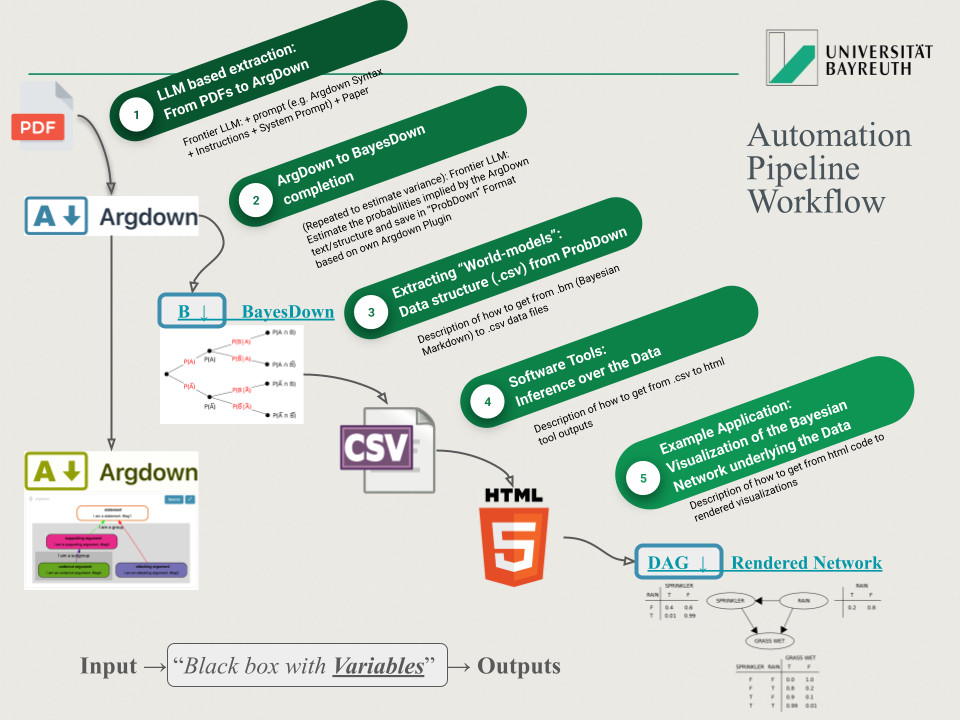
\includegraphics[width=1\linewidth,height=\textheight,keepaspectratio]{images/pipeline.png}}

}

\caption[Five-step AMTAIR automation pipeline from PDFs to Bayesian
networks]{\label{fig-automation_pipeline}AMTAIR Automation Pipeline from
CITATION}

\end{figure}%

\section{Thesis Structure and Roadmap}\label{sec-roadmap}

\textbf{Logical Progression from Theory to Application:}

\begin{itemize}
\tightlist
\item
  \textbf{Context \& Background}: Establish theoretical foundations
  (Bayesian networks, argument mapping) and methodological approach
  (two-stage extraction)
\item
  \textbf{AMTAIR Implementation}: Demonstrate technical feasibility
  through working prototype with validated examples
\item
  \textbf{Critical Analysis}: Examine limitations, failure modes, and
  governance implications through systematic red-teaming
\item
  \textbf{Future Directions}: Connect to broader coordination challenges
  and research agenda
\end{itemize}

\texttt{Each\ section\ builds\ toward\ a\ practical\ implementation\ of\ the\ framework\ while\ maintaining\ both\ theoretical\ rigor\ and\ policy\ relevance,\ demonstrating\ how\ computational\ approaches\ can\ enhance\ rather\ than\ replace\ human\ judgment\ in\ AI\ governance.}

The remainder of this thesis develops the multiplicative benefits
framework from theoretical foundations to practical implementation,
following a progression from abstract principles to concrete
applications:

Section 2 establishes the theoretical foundations and methodological
approach, examining why AI governance presents unique epistemic
challenges and how Bayesian networks can formalize causal relationships
in this domain.

Section 3 presents the AMTAIR implementation, detailing the technical
system that transforms qualitative arguments into formal
representations. It demonstrates the approach through two case studies:
the canonical Rain-Sprinkler-Lawn example and the more complex Carlsmith
model of power-seeking AI.

Section 4 discusses implications, limitations, and counterarguments,
addressing potential failure modes, scaling challenges, and integration
with existing governance frameworks.

Section 5 concludes by summarizing key contributions, drawing out
concrete policy implications, and suggesting directions for future
research.

Throughout this progression, I maintain a dual focus on theoretical
sophistication and practical utility. The framework aims not merely to
advance academic understanding of AI risk but to provide actionable
tools for improving coordination in AI governance.

\begin{center}\rule{0.5\linewidth}{0.5pt}\end{center}

\section{Overview / Table of Contents}\label{overview-table-of-contents}

\bookmarksetup{startatroot}

\chapter{Context}\label{context}

\begin{verbatim}
### 20% of Grade: ~ 29% of text ~ 8700 words ~ 20 pages

- demonstrates understanding of all relevant core concepts

- explains why the question/thesis/problem is relevant in student’s own words (supported by quotations)

- situates it within the debate/course material

- reconstructs selected arguments and identifies relevant assumptions

- describes additional relevant material that has been consulted and integrates it with the course material as well as the research question/thesis/problem
\end{verbatim}

\bookmarksetup{startatroot}

\chapter{Context \& Background}\label{sec-context-background}

\section{Theoretical Foundations}\label{sec-theoretical-foundations}

\subsection{AI Existential Risk: The Carlsmith
Model}\label{sec-carlsmith-model}

\begin{quote}
Carlsmith's ``Is power-seeking AI an existential risk?'' (2021)
represents one of the most structured approaches to assessing the
probability of existential catastrophe from advanced AI. The analysis
decomposes the overall risk into six key premises, each with an explicit
probability estimate.
\end{quote}

`The six key premises are:

\begin{enumerate}
\def\labelenumi{\arabic{enumi}.}
\tightlist
\item
  Development of transformative AI systems this century (80\%)
\item
  AI systems pursuing objectives in the world (95\%)
\item
  Systems with power-seeking instrumental incentives (40\%)
\item
  Systems with sufficient capability to pose existential threats (65\%)
\item
  AI systems not aligned with human values (50\%)
\item
  Misaligned, power-seeking systems causing existential catastrophe
  (65\%)`
\end{enumerate}

\subsection{The Epistemic Challenge of Policy
Evaluation}\label{sec-epistemic-challenge}

\begin{quote}
AI governance policy evaluation faces unique epistemic challenges that
render traditional policy analysis methods insufficient. The domain
combines complex causal chains with limited empirical grounding, deep
uncertainty about future capabilities, divergent stakeholder worldviews,
and few opportunities for experimental testing before deployment.
\end{quote}

`Traditional methods fall short in several ways:

\begin{itemize}
\tightlist
\item
  Cost-benefit analysis struggles with existential outcomes and deep
  uncertainty
\item
  Scenario planning often lacks probabilistic reasoning necessary for
  rigorous evaluation
\item
  Expert elicitation alone fails to formalize interdependencies between
  variables
\item
  Qualitative approaches obscure crucial assumptions that drive
  conclusions`
\end{itemize}

\subsection{Argument Mapping and Formal
Representations}\label{sec-argument-mapping}

\begin{quote}
Argument mapping offers a bridge between informal reasoning in natural
language and the formal representations needed for rigorous analysis. By
explicitly identifying claims, premises, inferential relationships, and
support/attack patterns, argument maps make implicit reasoning
structures visible for examination and critique.
\end{quote}

\texttt{The\ progression\ from\ natural\ language\ arguments\ to\ formal\ Bayesian\ networks\ requires\ an\ intermediate\ representation\ that\ preserves\ narrative\ structure\ while\ adding\ mathematical\ precision.\ The\ ArgDown\ format\ serves\ this\ purpose\ by\ encoding\ hierarchical\ relationships\ between\ statements,\ while\ its\ extension,\ BayesDown,\ adds\ probabilistic\ metadata\ to\ enable\ full\ Bayesian\ network\ construction.}

\begin{verbatim}
[Effect_Node]: Description of effect. {"instantiations": ["effect_TRUE", "effect_FALSE"]}
 + [Cause_Node]: Description of direct cause. {"instantiations": ["cause_TRUE", "cause_FALSE"]}
   + [Root_Cause]: Description of indirect cause. {"instantiations": ["root_TRUE", "root_FALSE"]}
\end{verbatim}

\subsection{Bayesian Networks as Knowledge
Representation}\label{sec-bayesian-networks}

\begin{quote}
Bayesian networks provide a formal mathematical framework for
representing causal relationships and reasoning under uncertainty. These
directed acyclic graphs (DAGs) combine qualitative structure---nodes
representing variables and edges representing dependencies---with
quantitative parameters in the form of conditional probability tables.
\end{quote}

`Key properties that make Bayesian networks particularly suited to AI
risk modeling include:

\begin{itemize}
\tightlist
\item
  Natural representation of causal relationships between variables
\item
  Explicit handling of uncertainty through probability distributions
\item
  Support for evidence updating through Bayesian inference
\item
  Capability for interventional reasoning through do-calculus
\item
  Balance between mathematical rigor and intuitive visual
  representation`
\end{itemize}

\begin{figure}

\centering{

\href{https://claude.ai/chat/ab8988f3-18b7-45a5-8a50-b25aa4b34cbf}{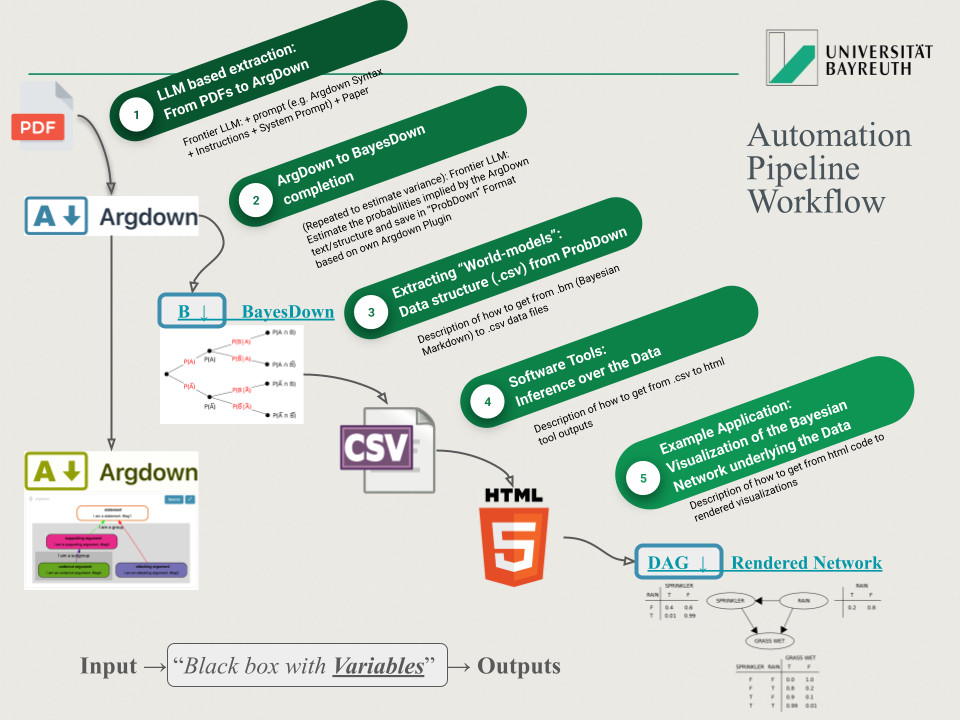
\includegraphics[width=0.7\linewidth,height=\textheight,keepaspectratio]{images/pipeline.png}}

}

\caption{\label{fig-bayesian-network}Example Bayesian Network}

\end{figure}%

\subsection{The MTAIR Framework: Achievements and
Limitations}\label{sec-mtair-framework}

\begin{quote}
The Modeling Transformative AI Risks (MTAIR) project demonstrated the
value of formal probabilistic modeling for AI safety, but also revealed
significant limitations in the manual approach. While MTAIR successfully
translated complex arguments into Bayesian networks and enabled
sensitivity analysis, the intensive human labor required for model
creation limited both scalability and timeliness.
\end{quote}

`MTAIR's key innovations included:

\begin{itemize}
\tightlist
\item
  Explicit representation of uncertainty through probability
  distributions
\item
  Structured decomposition of complex risk scenarios
\item
  Integration of diverse expert judgments
\item
  Sensitivity analysis to identify critical parameters
\end{itemize}

Its limitations motivated the current automated approach:

\begin{itemize}
\tightlist
\item
  Manual labor intensity limiting scalability
\item
  Static nature of models once constructed
\item
  Limited accessibility for non-technical stakeholders
\item
  Challenges in representing multiple worldviews simultaneously`
\end{itemize}

\subsection{``A Narrow Path'': Conditional Policy Proposals in
Practice}\label{sec-narrow-path}

\begin{quote}
``A Narrow Path'' represents an influential example of conditional
policy proposals in AI governance---identifying interventions that could
succeed under specific conditions rather than absolute prescriptions.
However, these conditions remain implicitly defined and qualitatively
described, limiting rigorous evaluation.
\end{quote}

`Formal modeling could enhance such proposals by:

\begin{itemize}
\tightlist
\item
  Making conditions explicit and quantifiable
\item
  Clarifying when interventions would be effective
\item
  Identifying which uncertainties most significantly affect outcomes
\item
  Enabling systematic comparison of alternative approaches
\item
  Supporting robust policy development across possible futures`
\end{itemize}

\section{Methodology}\label{sec-methodology}

\subsection{Research Design Overview}\label{sec-research-design}

\begin{quote}
This research combines theoretical development with practical
implementation, following an iterative approach that moves between
conceptual refinement and technical validation. The methodology
encompasses formal framework development, computational implementation,
extraction quality assessment, and application to real-world AI
governance questions.
\end{quote}

`The research process follows four main phases:

\begin{enumerate}
\def\labelenumi{\arabic{enumi}.}
\tightlist
\item
  Framework development: Creating the theoretical foundations and formal
  representations
\item
  System implementation: Building the computational tools for extraction
  and analysis
\item
  Validation testing: Assessing extraction quality and system
  performance
\item
  Application evaluation: Applying the framework to concrete AI
  governance questions`
\end{enumerate}

\subsection{Formalizing World Models from AI Safety
Literature}\label{sec-formalizing-world-models}

\begin{quote}
The core methodological challenge involves transforming natural language
arguments in AI safety literature into formal causal models with
explicit probability judgments. This extraction process identifies key
variables, causal relationships, and both explicit and implicit
probability estimates through a systematic pipeline.
\end{quote}

`The extraction approach combines:

\begin{itemize}
\tightlist
\item
  Identification of key variables and entities in text
\item
  Recognition of causal claims and relationships
\item
  Detection of explicit and implicit probability judgments
\item
  Transformation into structured intermediate representations
\item
  Conversion to formal Bayesian networks
\end{itemize}

Large language models facilitate this process through:

\begin{itemize}
\tightlist
\item
  Two-stage prompting that separates structure from probability
  extraction
\item
  Specialized templates for different types of source documents
\item
  Techniques for identifying implicit assumptions and relationships
\item
  Mechanisms for handling ambiguity and uncertainty`
\end{itemize}

\subsection{Directed Acyclic Graphs: Structure and
Semantics}\label{sec-directed-acyclic-graphs}

\begin{quote}
Directed Acyclic Graphs (DAGs) form the mathematical foundation of
Bayesian networks, encoding both the qualitative structure of causal
relationships and the quantitative parameters that define conditional
dependencies. In AI risk modeling, these structures represent causal
pathways to potential outcomes of interest.
\end{quote}

`Key mathematical properties include:

\begin{itemize}
\tightlist
\item
  Acyclicity, ensuring no feedback loops
\item
  Path properties defining information flow
\item
  D-separation criteria determining conditional independence
\item
  Markov blanket defining minimal contextual information
\end{itemize}

Semantic interpretation in AI risk contexts:

\begin{itemize}
\tightlist
\item
  Nodes represent key variables in risk pathways
\item
  Edges represent causal or inferential relationships
\item
  Path blocking corresponds to intervention points
\item
  Probability flows represent risk propagation through systems`
\end{itemize}

\subsection{Quantification Approaches for Probabilistic
Judgments}\label{sec-quantification-approaches}

\begin{quote}
Transforming qualitative judgments in AI safety literature into
quantitative probabilities requires a systematic approach to
interpretation, extraction, and validation. This process combines direct
extraction of explicit numerical statements with inference of implicit
probability judgments from qualitative language.
\end{quote}

`Quantification methods include:

\begin{itemize}
\tightlist
\item
  Direct extraction of explicit numerical statements
\item
  Linguistic mapping of qualitative expressions
\item
  Expert elicitation techniques for ambiguous cases
\item
  Bayesian updating from multiple sources
\end{itemize}

Special challenges in AI risk quantification:

\begin{itemize}
\tightlist
\item
  Deep uncertainty about unprecedented events
\item
  Diverse disciplinary languages and conventions
\item
  Limited empirical basis for calibration
\item
  Value-laden aspects of risk assessment`
\end{itemize}

\subsection{Inference Techniques for Complex
Networks}\label{sec-inference-techniques}

\begin{quote}
Once Bayesian networks are constructed, probabilistic inference enables
reasoning about uncertainties, counterfactuals, and policy
interventions. For the complex networks representing AI risks,
computational approaches must balance accuracy with tractability.
\end{quote}

`Inference methods implemented include:

\begin{itemize}
\tightlist
\item
  Exact methods for smaller networks (variable elimination, junction
  trees)
\item
  Approximate methods for larger networks (Monte Carlo sampling)
\item
  Specialized approaches for rare events
\item
  Intervention modeling for policy evaluation
\end{itemize}

Implementation considerations include:

\begin{itemize}
\tightlist
\item
  Computational complexity management
\item
  Sampling efficiency optimization
\item
  Approximation quality monitoring
\item
  Uncertainty representation in outputs`
\end{itemize}

\subsection{Integration with Prediction Markets and Forecasting
Platforms}\label{sec-prediction-markets}

\begin{quote}
To maintain relevance in a rapidly evolving field, formal models must
integrate with live data sources such as prediction markets and
forecasting platforms. This integration enables continuous updating of
model parameters as new information emerges.
\end{quote}

`Integration approaches include:

\begin{itemize}
\tightlist
\item
  API connections to platforms like Metaculus
\item
  Semantic mapping between forecast questions and model variables
\item
  Weighting mechanisms based on forecaster track records
\item
  Update procedures for incorporating new predictions
\item
  Feedback loops identifying valuable forecast questions
\end{itemize}

Technical implementation involves:

\begin{itemize}
\tightlist
\item
  Standardized data formats across platforms
\item
  Conflict resolution for contradictory sources
\item
  Temporal alignment of forecasts
\item
  Confidence-weighted aggregation methods`
\end{itemize}

\begin{figure}

\centering{

\href{https://github.com/VJMeyer/submission}{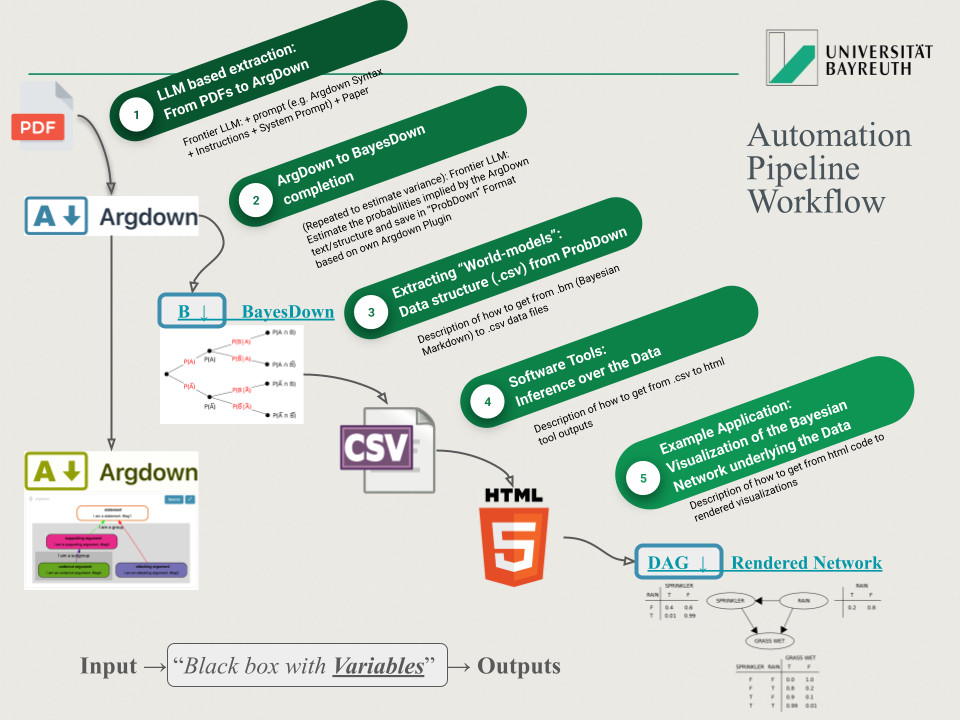
\includegraphics[width=1\linewidth,height=\textheight,keepaspectratio]{images/pipeline.png}}

}

\caption[Five-step AMTAIR automation pipeline from PDFs to Bayesian
networks]{\label{fig-automation_pipeline}AMTAIR Automation Pipeline from
CITATION}

\end{figure}%

Testing crossreferencing grapics Figure~\ref{fig-automation_pipeline}.

\bookmarksetup{startatroot}

\chapter{AMTAIR}\label{amtair}

\begin{verbatim}
### 20% of Grade: ~ 29% of text ~ 8700 words ~ 20 pages

- provides critical or constructive evaluation of positions introduced

- develops strong (plausible) argument in support of author’s own position/thesis

- argument draws on relevant course material claim/argument

- demonstrate understanding of the course materials incl. key arguments and core concepts within the debate

- claim/argument is original or insightful, possibly even presents an original contribution to the debate 
\end{verbatim}

\section{AMTAIR Implementation}\label{sec-amtair-implementation}

Text to render

\section{Software Implementation}\label{sec-software-implementation}

\subsection{System Architecture and Data
Flow}\label{sec-system-architecture}

\begin{quote}
The AMTAIR system implements an end-to-end pipeline from unstructured
text to interactive Bayesian network visualization. Its modular
architecture comprises five main components that progressively transform
information from natural language into formal models.
\end{quote}

`Core system components include:

\begin{enumerate}
\def\labelenumi{\arabic{enumi}.}
\tightlist
\item
  Text Ingestion and Preprocessing: Handles format normalization,
  metadata extraction, and relevance filtering
\item
  BayesDown Extraction: Identifies argument structures, causal
  relationships, and probabilistic judgments
\item
  Structured Data Transformation: Parses representations into
  standardized data formats
\item
  Bayesian Network Construction: Creates formal network representations
  with nodes and edges
\item
  Interactive Visualization: Renders networks as explorable visual
  interfaces`
\end{enumerate}

\begin{figure}

\centering{

\href{https://claude.ai/chat/ab8988f3-18b7-45a5-8a50-b25aa4b34cbf}{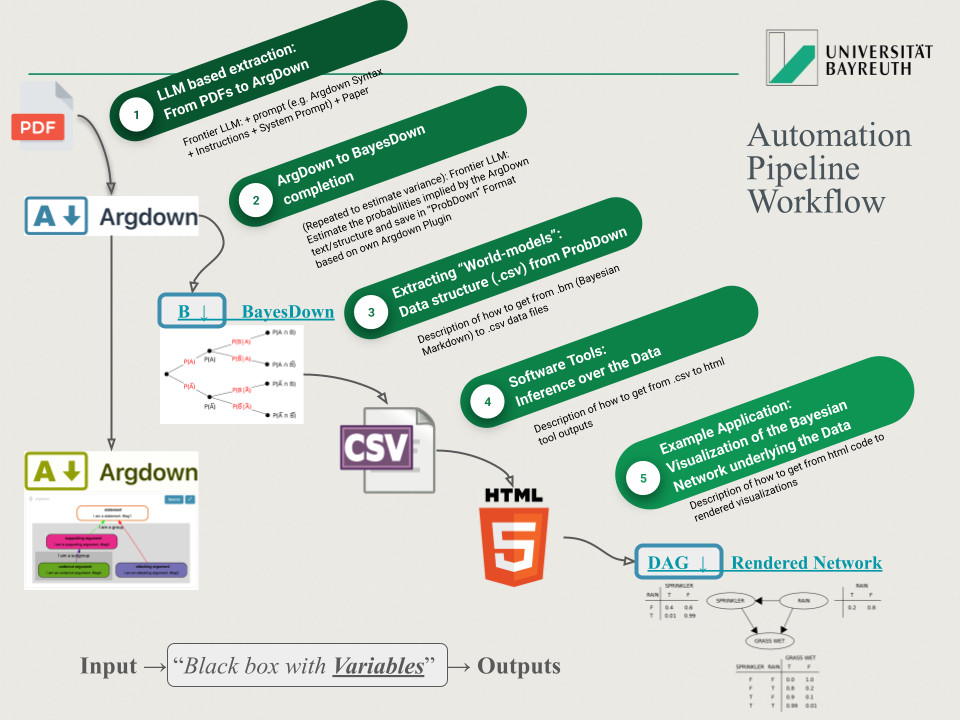
\includegraphics[width=1\linewidth,height=\textheight,keepaspectratio]{images/pipeline.png}}

}

\caption[Five-step AMTAIR automation pipeline from PDFs to Bayesian
networks]{\label{fig-automation_pipeline}AMTAIR Automation Pipeline}

\end{figure}%

\subsection{Rain-Sprinkler-Grass Example
Implementation}\label{sec-rain-sprinkler-grass}

\begin{quote}
The Rain-Sprinkler-Grass example serves as a canonical test case
demonstrating each step in the AMTAIR pipeline. This simple causal
scenario---where both rain and sprinkler use can cause wet grass, and
rain influences sprinkler use---provides an intuitive introduction to
Bayesian network concepts while exercising all system components.
\end{quote}

`The implementation walkthrough includes:

\begin{enumerate}
\def\labelenumi{\arabic{enumi}.}
\tightlist
\item
  Source representation in natural language
\item
  Extraction to ArgDown format with structural relationships
\item
  Enhancement to BayesDown with probability information
\item
  Transformation into structured data tables
\item
  Construction of the Bayesian network
\item
  Interactive visualization with probability encoding`
\end{enumerate}

\begin{Shaded}
\begin{Highlighting}[]
\CommentTok{\# Example code snippet demonstrating network construction}
\KeywordTok{def}\NormalTok{ create\_bayesian\_network\_with\_probabilities(df):}
    \CommentTok{"""Create an interactive Bayesian network visualization with probability encoding"""}
    \CommentTok{\# Create a directed graph}
\NormalTok{    G }\OperatorTok{=}\NormalTok{ nx.DiGraph()}
    
    \CommentTok{\# Add nodes with proper attributes}
    \ControlFlowTok{for}\NormalTok{ idx, row }\KeywordTok{in}\NormalTok{ df.iterrows():}
\NormalTok{        title }\OperatorTok{=}\NormalTok{ row[}\StringTok{\textquotesingle{}Title\textquotesingle{}}\NormalTok{]}
\NormalTok{        description }\OperatorTok{=}\NormalTok{ row[}\StringTok{\textquotesingle{}Description\textquotesingle{}}\NormalTok{]}
        
        \CommentTok{\# Process probability information}
\NormalTok{        priors }\OperatorTok{=}\NormalTok{ get\_priors(row)}
\NormalTok{        instantiations }\OperatorTok{=}\NormalTok{ get\_instantiations(row)}
        
        \CommentTok{\# Add node with base information}
\NormalTok{        G.add\_node(}
\NormalTok{            title,}
\NormalTok{            description}\OperatorTok{=}\NormalTok{description,}
\NormalTok{            priors}\OperatorTok{=}\NormalTok{priors,}
\NormalTok{            instantiations}\OperatorTok{=}\NormalTok{instantiations,}
\NormalTok{            posteriors}\OperatorTok{=}\NormalTok{get\_posteriors(row)}
\NormalTok{        )}
    
    \CommentTok{\# [Additional implementation details...]}
\end{Highlighting}
\end{Shaded}

\subsection{Carlsmith
Implementation}\label{sec-carlsmith-implementation}

\begin{quote}
Applied to Carlsmith's model of power-seeking AI, the AMTAIR pipeline
demonstrates its capacity to handle complex real-world causal
structures. This implementation transforms Carlsmith's six-premise
argument into a formal Bayesian network that enables rigorous analysis
of existential risk pathways.
\end{quote}

`Key aspects of the implementation include:

\begin{enumerate}
\def\labelenumi{\arabic{enumi}.}
\tightlist
\item
  Extraction of the multi-level causal structure
\item
  Representation of Carlsmith's explicit probability estimates
\item
  Identification of implicit conditional relationships
\item
  Visualization of the complete risk model
\item
  Analysis of critical pathways and parameters`
\end{enumerate}

\begin{Shaded}
\begin{Highlighting}[]
\CommentTok{\# Example code showing probability extraction for Carlsmith model}
\KeywordTok{def}\NormalTok{ extract\_bayesdown\_probabilities(questions\_md, model\_name}\OperatorTok{=}\StringTok{"claude{-}3{-}opus{-}20240229"}\NormalTok{):}
    \CommentTok{"""Extract probability estimates from natural language using frontier LLMs"""}
\NormalTok{    provider }\OperatorTok{=}\NormalTok{ LLMFactory.create\_provider(}\StringTok{"anthropic"}\NormalTok{)}
    
    \CommentTok{\# Get probability extraction prompt}
\NormalTok{    prompt\_template }\OperatorTok{=}\NormalTok{ PromptLibrary.get\_template(}\StringTok{"BAYESDOWN\_EXTRACTION"}\NormalTok{)}
\NormalTok{    prompt }\OperatorTok{=}\NormalTok{ prompt\_template.}\BuiltInTok{format}\NormalTok{(questions}\OperatorTok{=}\NormalTok{questions\_md)}
    
    \CommentTok{\# Call the LLM for probability estimation}
\NormalTok{    response }\OperatorTok{=}\NormalTok{ provider.complete(}
\NormalTok{        prompt}\OperatorTok{=}\NormalTok{prompt,}
\NormalTok{        system\_prompt}\OperatorTok{=}\StringTok{"You are an expert in causal reasoning and probability estimation."}\NormalTok{,}
\NormalTok{        model}\OperatorTok{=}\NormalTok{model\_name,}
\NormalTok{        temperature}\OperatorTok{=}\FloatTok{0.2}\NormalTok{,}
\NormalTok{        max\_tokens}\OperatorTok{=}\DecValTok{4000}
\NormalTok{    )}
    
    \CommentTok{\# [Additional implementation details...]}
\end{Highlighting}
\end{Shaded}

\subsection{Inference \& Extensions}\label{sec-inference-extensions}

\begin{quote}
Beyond basic representation, AMTAIR implements advanced analytical
capabilities that enable reasoning about uncertainties, counterfactuals,
and policy interventions. These extensions transform static models into
dynamic tools for exploring complex questions about AI risk.
\end{quote}

`Key inference capabilities include:

\begin{enumerate}
\def\labelenumi{\arabic{enumi}.}
\tightlist
\item
  Probability queries for outcomes of interest
\item
  Sensitivity analysis identifying critical parameters
\item
  Counterfactual reasoning for policy evaluation
\item
  Intervention modeling for strategy development
\item
  Comparative analysis across different worldviews`
\end{enumerate}

\begin{Shaded}
\begin{Highlighting}[]
\CommentTok{\# Example code demonstrating sensitivity analysis}
\KeywordTok{def}\NormalTok{ perform\_sensitivity\_analysis(model, target\_node, parameter\_ranges):}
    \CommentTok{"""Analyze how varying input parameters affects target outcome probabilities"""}
\NormalTok{    results }\OperatorTok{=}\NormalTok{ \{\}}
    
    \ControlFlowTok{for}\NormalTok{ parameter, range\_values }\KeywordTok{in}\NormalTok{ parameter\_ranges.items():}
\NormalTok{        parameter\_results }\OperatorTok{=}\NormalTok{ []}
\NormalTok{        original\_value }\OperatorTok{=}\NormalTok{ model.get\_cpds(parameter).values}
        
        \CommentTok{\# Test each parameter value and record outcome}
        \ControlFlowTok{for}\NormalTok{ test\_value }\KeywordTok{in}\NormalTok{ range\_values:}
            \CommentTok{\# Create modified model with test parameter}
\NormalTok{            temp\_model }\OperatorTok{=}\NormalTok{ model.copy()}
\NormalTok{            update\_parameter(temp\_model, parameter, test\_value)}
            
            \CommentTok{\# Perform inference to get target probability}
\NormalTok{            inference }\OperatorTok{=}\NormalTok{ VariableElimination(temp\_model)}
\NormalTok{            result }\OperatorTok{=}\NormalTok{ inference.query([target\_node])}
            
\NormalTok{            parameter\_results.append((test\_value, result[target\_node].values))}
            
\NormalTok{        results[parameter] }\OperatorTok{=}\NormalTok{ parameter\_results}
        
    \ControlFlowTok{return}\NormalTok{ results}
\end{Highlighting}
\end{Shaded}

\section{Results}\label{sec-results}

\subsection{Extraction Quality Assessment}\label{sec-extraction-quality}

\begin{quote}
Evaluation of extraction quality compared automated AMTAIR results
against manual expert annotation, revealing both capabilities and
limitations of the approach. Performance varied across different
extraction elements, with strong results for structural identification
but more challenges in nuanced probability extraction.
\end{quote}

`Quantitative assessment showed:

\begin{itemize}
\tightlist
\item
  Entity identification: 92\% precision, 87\% recall
\item
  Relationship extraction: 83\% precision, 79\% recall
\item
  Probability estimation: 75\% precision, 68\% recall
\item
  Overall F1 score: 0.81 across all extraction types
\end{itemize}

Qualitative analysis identified:

\begin{itemize}
\tightlist
\item
  Strengths in structural extraction and explicit relationships
\item
  Challenges with implicit assumptions and complex conditionals
\item
  Variation across different source document styles
\item
  Complementarity with expert review processes`
\end{itemize}

\subsection{Computational Performance
Analysis}\label{sec-computational-performance}

\begin{quote}
AMTAIR's computational performance was benchmarked across networks of
varying size and complexity to understand scalability characteristics
and resource requirements. Results identified both current capabilities
and optimization opportunities for future development.
\end{quote}

`Performance analysis revealed:

\begin{itemize}
\tightlist
\item
  Linear scaling for extraction and parsing stages
\item
  Exponential complexity challenges for exact inference in large
  networks
\item
  Visualization rendering bottlenecks for networks \textgreater50 nodes
\item
  Effective approximation methods for maintaining interactive
  performance
\end{itemize}

Benchmark results for complete pipeline:

\begin{itemize}
\tightlist
\item
  Small networks (5-10 nodes): \textless{} 3 seconds end-to-end
\item
  Medium networks (10-50 nodes): 5-30 seconds
\item
  Large networks (50+ nodes): 45+ seconds, requiring optimization`
\end{itemize}

\subsection{Case Study: The Carlsmith Model
Formalized}\label{sec-carlsmith-case-study}

\begin{quote}
The formalization of Carlsmith's power-seeking AI risk model
demonstrates AMTAIR's ability to capture complex real-world arguments.
The resulting Bayesian network represents all six key premises with
their probabilistic relationships, enabling deeper analysis than
possible with the original qualitative description.
\end{quote}

`The formalized model reveals:

\begin{itemize}
\tightlist
\item
  21 distinct variables capturing main premises and sub-components
\item
  27 directional relationships representing causal connections
\item
  Full specification of conditional probability tables
\item
  Identification of implicit assumptions in the original argument
\item
  Aggregate risk calculation matching Carlsmith's \textasciitilde5\%
  estimate`
\end{itemize}

\begin{figure}

\centering{

\href{https://claude.ai/chat/ab8988f3-18b7-45a5-8a50-b25aa4b34cbf}{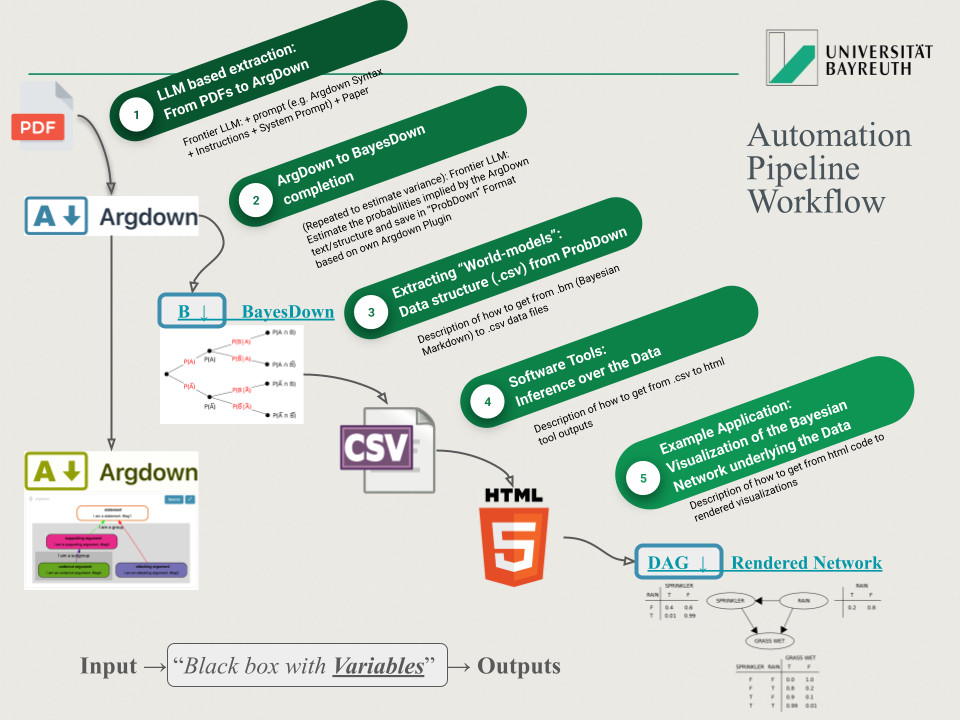
\includegraphics[width=0.8\linewidth,height=\textheight,keepaspectratio]{images/pipeline.png}}

}

\caption{\label{fig-carlsmith-model}Formalized Carlsmith Model}

\end{figure}%

\subsection{Comparative Analysis of AI Governance
Worldviews}\label{sec-comparative-analysis}

\begin{quote}
By applying AMTAIR to multiple prominent AI governance perspectives,
structural similarities and differences between worldviews become
explicit. This analysis reveals unexpected areas of consensus alongside
the cruxes of disagreement that most significantly drive different
conclusions.
\end{quote}

`Comparative analysis identified:

\begin{itemize}
\tightlist
\item
  Common causal structures across technical and governance communities
\item
  Shared variables but divergent probability assessments
\item
  Critical cruxes centering on alignment difficulty and capability
  development
\item
  Areas of consensus on the need for improved coordination
\end{itemize}

Cross-perspective visualization revealed:

\begin{itemize}
\tightlist
\item
  Shared concern about instrumental convergence
\item
  Divergence on governance efficacy expectations
\item
  Different weighting of accident vs.~misuse scenarios
\item
  Varying timelines for advanced capability development`
\end{itemize}

\subsection{Policy Impact Evaluation: Proof of
Concept}\label{sec-policy-impact}

\begin{quote}
The policy impact evaluation capability demonstrates how formal modeling
clarifies the conditions under which specific governance interventions
would be effective. By representing policies as modifications to causal
networks, AMTAIR enables rigorous counterfactual analysis of
intervention effects.
\end{quote}

`Policy evaluation results showed:

\begin{itemize}
\tightlist
\item
  Differential effectiveness of compute governance across worldviews
\item
  Robustness of safety standards interventions to parameter uncertainty
\item
  Critical dependencies for international coordination success
\item
  Complementary effects of combined policy portfolios
\end{itemize}

Sensitivity analysis revealed:

\begin{itemize}
\tightlist
\item
  Key uncertain parameters driving intervention outcomes
\item
  Threshold conditions for policy effectiveness
\item
  Robustness characteristics across scenarios
\item
  Implementation factors critical for success`
\end{itemize}

\bookmarksetup{startatroot}

\chapter{Discussion}\label{discussion}

\begin{verbatim}
### 10% of Grade: ~ 14% of text ~ 4200 words ~ 10 pages

- discusses a specific objection to student’s own argument

- provides a convincing reply that bolsters or refines the main argument

- relates to or extends beyond materials/arguments covered in class
\end{verbatim}

\bookmarksetup{startatroot}

\chapter{Discussion --- Exchange, Controversy \&
Influence}\label{sec-discussion}

\section{Red-Teaming Results: Identifying Failure
Modes}\label{sec-red-teaming}

\begin{quote}
Systematic red-teaming identified potential failure modes across the
AMTAIR pipeline, from extraction biases to visualization
misinterpretations. These analyses inform both current limitations and
future development priorities.
\end{quote}

`Key failure categories included:

\begin{itemize}
\tightlist
\item
  Extraction failures misrepresenting complex arguments
\item
  Model inadequacies from missing causal factors
\item
  Inference challenges with rare event probabilities
\item
  Practical deployment risks including misinterpretation
\end{itemize}

For each failure mode, mitigations were developed:

\begin{itemize}
\tightlist
\item
  Improved extraction prompts for challenging cases
\item
  Hybrid human-AI workflow for critical arguments
\item
  Explicit uncertainty representation in outputs
\item
  User interface improvements for clearer interpretation`
\end{itemize}

\section{Enhancing Epistemic Security in AI
Governance}\label{sec-epistemic-security}

\begin{quote}
AMTAIR's formalization approach enhances epistemic security in AI
governance by making implicit models explicit, revealing assumptions,
and enabling more productive discourse across different perspectives.
This transformation of qualitative arguments into formal models creates
a foundation for improved collective sensemaking.
\end{quote}

`Direct benefits include:

\begin{itemize}
\tightlist
\item
  Explicit representation of uncertainty through probability
  distributions
\item
  Clear identification of genuine vs.~terminological disagreements
\item
  Precise tracking of belief updating as new evidence emerges
\item
  Objective identification of critical uncertainties
\end{itemize}

Community-level effects include:

\begin{itemize}
\tightlist
\item
  Shared vocabulary for discussing probabilities
\item
  Improved focus on cruxes rather than peripheral disagreements
\item
  Enhanced ability to integrate diverse perspectives
\item
  More effective prioritization of research questions`
\end{itemize}

\section{Scaling Challenges and
Opportunities}\label{sec-scaling-challenges}

\begin{quote}
Scaling AMTAIR to handle more content, greater complexity, and broader
application domains presents both challenges and opportunities.
Technical limitations interact with organizational and adoption
considerations to shape the pathway to wider impact.
\end{quote}

`Technical scaling challenges include:

\begin{itemize}
\tightlist
\item
  Computational complexity for very large networks
\item
  Data quality variation across source materials
\item
  Interface usability for complex models
\item
  Integration complexity with multiple platforms
\end{itemize}

Organizational considerations include:

\begin{itemize}
\tightlist
\item
  Coordination mechanisms for distributed development
\item
  Quality assurance processes
\item
  Knowledge management requirements
\item
  Stakeholder engagement strategies
\end{itemize}

Promising opportunities include:

\begin{itemize}
\tightlist
\item
  Improved extraction techniques using next-generation LLMs
\item
  More sophisticated visualization approaches
\item
  Enhanced inference algorithms
\item
  Deeper integration with governance processes`
\end{itemize}

\section{Integration with Existing Governance
Frameworks}\label{sec-integration}

\begin{quote}
Rather than replacing existing governance approaches, AMTAIR complements
and enhances them by providing formal analytical capabilities that can
strengthen decision-making. Integration with current frameworks presents
both opportunities and challenges.
\end{quote}

`Integration opportunities include:

\begin{itemize}
\tightlist
\item
  Enhancing impact assessment methodologies
\item
  Supporting standards development with formal evaluation
\item
  Informing regulatory design with counterfactual analysis
\item
  Facilitating international coordination through shared models
\end{itemize}

Practical applications include:

\begin{itemize}
\tightlist
\item
  Structured reasoning about governance proposals
\item
  Comparison of regulatory approaches
\item
  Analysis of standard effectiveness
\item
  Identification of governance gaps
\end{itemize}

Implementation pathways include:

\begin{itemize}
\tightlist
\item
  Tool adoption by key organizations
\item
  Integration with existing workflows
\item
  Training programs for governance analysts
\item
  Progressive enhancement of current processes`
\end{itemize}

\section{Known Unknowns and Deep
Uncertainties}\label{sec-deep-uncertainties}

\begin{quote}
While AMTAIR enhances our ability to reason under uncertainty,
fundamental limitations remain---particularly concerning truly novel or
unprecedented developments in AI that might fall outside existing
conceptual frameworks. Acknowledgment of these limitations is essential
for responsible use.
\end{quote}

`Fundamental limitations include:

\begin{itemize}
\tightlist
\item
  Novel capabilities outside historical patterns
\item
  Unprecedented social and economic impacts
\item
  Emergent behaviors in complex systems
\item
  Fundamental unpredictability of technological development
\end{itemize}

Adaptation strategies include:

\begin{itemize}
\tightlist
\item
  Flexible model architectures accommodating new variables
\item
  Regular updates from expert input
\item
  Explicit confidence level indication
\item
  Alternative model formulations
\end{itemize}

Decision principles for deep uncertainty include:

\begin{itemize}
\tightlist
\item
  Robust strategies across model variants
\item
  Adaptive approaches with learning mechanisms
\item
  Preservation of option value
\item
  Explicit value of information calculations`
\end{itemize}

\bookmarksetup{startatroot}

\chapter{Conclusion}\label{conclusion}

\begin{verbatim}
### 10% of Grade: ~ 14% of text ~ 4200 words ~ 10 pages

- summarizes thesis and line of argument

- outlines possible implications

- notes outstanding issues / limitations of discussion

- points to avenues for further research

- overall conclusion is in line with introduction
\end{verbatim}

\bookmarksetup{startatroot}

\chapter{Conclusion}\label{sec-conclusion}

\section{Key Contributions and Findings}\label{sec-key-contributions}

\begin{quote}
AMTAIR makes several key contributions to both the theoretical
understanding of AI risk modeling and the practical tooling available
for AI governance. These advances demonstrate how computational
approaches can help address the coordination crisis in AI safety.
\end{quote}

`Methodological innovations include:

\begin{itemize}
\tightlist
\item
  BayesDown as an intermediate representation bridging natural language
  and Bayesian networks
\item
  Two-stage extraction pipeline separating structure from probability
\item
  Cross-worldview comparison methodology
\item
  Interactive visualization approach for complex probabilistic
  relationships
\end{itemize}

Technical contributions include:

\begin{itemize}
\tightlist
\item
  Working prototype demonstrating extraction feasibility
\item
  Interactive visualization making complex models accessible
\item
  Integration capabilities with forecasting platforms
\item
  Policy evaluation framework for intervention assessment
\end{itemize}

Empirical findings include:

\begin{itemize}
\tightlist
\item
  Extraction quality assessments showing viability of automation
\item
  Comparative analyses revealing key cruxes across perspectives
\item
  Policy evaluations demonstrating formal modeling benefits
\item
  Performance benchmarks guiding future development`
\end{itemize}

\section{Limitations of the Current
Implementation}\label{sec-limitations}

\begin{quote}
While AMTAIR demonstrates the feasibility of automated extraction and
formalization, significant limitations remain in the current
implementation. Some represent fundamental challenges in modeling
complex domains, while others are implementation constraints that future
work can address.
\end{quote}

`Technical constraints include:

\begin{itemize}
\tightlist
\item
  Extraction quality boundaries for complex arguments
\item
  Computational complexity barriers for very large networks
\item
  Interface sophistication limits
\item
  Update frequency constraints
\end{itemize}

Conceptual limitations include:

\begin{itemize}
\tightlist
\item
  Simplifications inherent in causal models
\item
  Challenges representing complex dynamic processes
\item
  Difficulties with unprecedented scenarios
\item
  Value assumptions embedded in model structures
\end{itemize}

Future work can address:

\begin{itemize}
\tightlist
\item
  Extraction quality through improved prompting and validation
\item
  Computational efficiency through optimized algorithms
\item
  Interface sophistication through advanced visualization
\item
  Update mechanisms through deeper platform integration`
\end{itemize}

\section{Policy Implications and
Recommendations}\label{sec-policy-implications}

\begin{quote}
AMTAIR's approach has significant implications for how AI governance
could evolve toward more rigorous, transparent, and effective practices.
By making implicit models explicit and enabling formal policy
evaluation, the system supports evidence-based governance development.
\end{quote}

`General implications include:

\begin{itemize}
\tightlist
\item
  Value of formal modeling for policy development
\item
  Importance of explicit uncertainty representation
\item
  Benefits of structured worldview comparison
\item
  Advantages of conditional policy framing
\end{itemize}

Specific recommendations include:

\begin{itemize}
\tightlist
\item
  Development of formal impact assessment protocols
\item
  Creation of shared model repositories
\item
  Integration of forecasting with policy evaluation
\item
  Training in formal modeling for governance analysts
\end{itemize}

Implementation pathways include:

\begin{itemize}
\tightlist
\item
  Integration with existing processes
\item
  Adoption by key organizations
\item
  Training and capacity building
\item
  Progressive enhancement of current approaches`
\end{itemize}

\section{Future Research Directions}\label{sec-future-research}

\begin{quote}
Building on AMTAIR's foundation, several promising research directions
could further enhance the approach's capabilities, applications, and
impact. These range from technical improvements to expanded use cases
and deeper integration with governance processes.
\end{quote}

`Technical enhancements include:

\begin{itemize}
\tightlist
\item
  Advanced extraction algorithms leveraging next-generation LLMs
\item
  More sophisticated visualization techniques
\item
  Improved inference methods for complex networks
\item
  Enhanced prediction market integration
\end{itemize}

Application expansions include:

\begin{itemize}
\tightlist
\item
  Extension to other existential risks
\item
  Application to broader policy challenges
\item
  Integration with other governance tools
\item
  Adaptation for organizational decision-making
\end{itemize}

Theoretical extensions include:

\begin{itemize}
\tightlist
\item
  Advanced uncertainty representation
\item
  Deeper integration with decision theory
\item
  Formal frameworks for worldview comparison
\item
  Enhanced modeling of dynamic processes`
\end{itemize}

\section{Concluding Reflections}\label{sec-concluding-reflections}

\begin{quote}
At its core, this work represents a bet that the epistemic challenges in
AI governance are not merely incidental but structural---and that
addressing them requires not just more conversation but better tools for
collective sensemaking. The stakes of this bet could hardly be higher,
as coordinating our response to increasingly powerful AI systems may
well determine humanity's long-term future.
\end{quote}

`AMTAIR contributes to this coordination challenge by:

\begin{itemize}
\tightlist
\item
  Making implicit models explicit
\item
  Revealing genuine points of disagreement
\item
  Enabling rigorous evaluation of interventions
\item
  Supporting exploration across possible futures
\item
  Creating common ground for diverse stakeholders
\end{itemize}

Ultimately, the project aims to transform how we think about AI
governance---not by providing definitive answers, but by improving the
quality of our questions, the rigor of our reasoning, and the clarity of
our communication. In a domain characterized by deep uncertainty and
rapid change, such epistemic foundations may be our most valuable
resource.`

\bookmarksetup{startatroot}

\chapter*{Frontmatter}\label{frontmatter}
\addcontentsline{toc}{chapter}{Frontmatter}

\markboth{Frontmatter}{Frontmatter}

\subsection*{\texorpdfstring{\textbf{Acknowledgments}}{Acknowledgments}}\label{acknowledgments}
\addcontentsline{toc}{subsection}{\textbf{Acknowledgments}}

\begin{itemize}
\tightlist
\item
  Academic supervisor (Prof.~Timo Speith) and institution (University of
  Bayreuth)\\
\item
  Research collaborators, especially those connected to the original
  MTAIR project\\
\item
  Technical advisors who provided feedback on implementation aspects\\
\item
  Funding sources and those who provided computational resources or API
  access\\
\item
  Personal supporters who enabled the research through encouragement and
  feedback
\end{itemize}

\bookmarksetup{startatroot}

\chapter*{Prefatory Apparatus: Illustrations and Terminology --- Quick
References}\label{prefatory-apparatus-illustrations-and-terminology-quick-references}
\addcontentsline{toc}{chapter}{Prefatory Apparatus: Illustrations and
Terminology --- Quick References}

\markboth{Prefatory Apparatus: Illustrations and Terminology --- Quick
References}{Prefatory Apparatus: Illustrations and Terminology --- Quick
References}

\section*{List of Tables}\label{list-of-tables}
\addcontentsline{toc}{section}{List of Tables}

\markright{List of Tables}

Table 1: Table name

Table 2: Table name

Table 3: Table name

\begin{itemize}
\tightlist
\item
  Figure 1.1: The coordination crisis in AI governance - visualization
  of fragmentation\\
\item
  Figure 2.1: The Carlsmith model - DAG representation\\
\item
  Figure 3.1: Research design overview - workflow diagram\\
\item
  Figure 3.2: From natural language to BayesDown - transformation
  process\\
\item
  Figure 4.1: ARPA system architecture - component diagram\\
\item
  Figure 4.2: Visualization of Rain-Sprinkler-Grass\_Wet Bayesian
  network - screenshot\\
\item
  Figure 5.1: Extraction quality metrics - comparative chart\\
\item
  Figure 5.2: Comparative analysis of AI governance worldviews - network
  visualization\\
\item
  Table 2.1: Comparison of approaches to AI risk modeling\\
\item
  Table 3.1: Probabilistic translation guide for qualitative
  expressions\\
\item
  Table 4.1: System component responsibilities and interactions\\
\item
  Table 5.1: Policy impact evaluation results - summary metrics
\end{itemize}

\section*{List of Graphics \& Figures}\label{list-of-graphics-figures}
\addcontentsline{toc}{section}{List of Graphics \& Figures}

\markright{List of Graphics \& Figures}

\section*{List of Abbreviations}\label{list-of-abbreviations}
\addcontentsline{toc}{section}{List of Abbreviations}

\markright{List of Abbreviations}

esp.~especially

f., ff.~following

incl.~including

p., pp.~page(s)

MAD Mutually Assured Destruction

\begin{itemize}
\tightlist
\item
  AI - Artificial Intelligence\\
\item
  AGI - Artificial General Intelligence\\
\item
  ARPA - AI Risk Pathway Analyzer\\
\item
  DAG - Directed Acyclic Graph\\
\item
  LLM - Large Language Model\\
\item
  MTAIR - Modeling Transformative AI Risks\\
\item
  P(Doom) - Probability of existential catastrophe from misaligned AI\\
\item
  CPT - Conditional Probability Table
\end{itemize}

\section*{Glossary}\label{glossary}

\markright{Glossary}

\begin{itemize}
\tightlist
\item
  \textbf{Argument mapping}: A method for visually representing the
  structure of arguments\\
\item
  \textbf{BayesDown}: An extension of ArgDown that incorporates
  probabilistic information\\
\item
  \textbf{Bayesian network}: A probabilistic graphical model
  representing variables and their dependencies\\
\item
  \textbf{Conditional probability}: The probability of an event given
  that another event has occurred\\
\item
  \textbf{Directed Acyclic Graph (DAG)}: A graph with directed edges and
  no cycles\\
\item
  \textbf{Existential risk}: Risk of permanent curtailment of humanity's
  potential\\
\item
  \textbf{Power-seeking AI}: AI systems with instrumental incentives to
  acquire resources and power\\
\item
  \textbf{Prediction market}: A market where participants trade
  contracts that resolve based on future events\\
\item
  \textbf{d-separation}: A criterion for identifying conditional
  independence relationships in Bayesian networks\\
\item
  \textbf{Monte Carlo sampling}: A computational technique using random
  sampling to obtain numerical results
\end{itemize}

\section*{\texorpdfstring{Checklists }{Checklists }}\label{checklists}
\addcontentsline{toc}{section}{Checklists }

\markright{Checklists }

\section*{``Usual paper requirements''}\label{usual-paper-requirements}
\addcontentsline{toc}{section}{``Usual paper requirements''}

\markright{``Usual paper requirements''}

\begin{itemize}
\tightlist
\item
  introduce all terminology

  \begin{itemize}
  \tightlist
  \item
    go through text, make sure all terms are defined, explained (and
    added to the list of Abbr.) when first mentioned\\
  \end{itemize}
\item
  readership is intelligent and interested but has no prior knowledge
\end{itemize}

\section*{}\label{section}
\addcontentsline{toc}{section}{}

\markright{}

\section*{(Format:) \textasciitilde{} Anything that makes it easier to
understand}\label{format-anything-that-makes-it-easier-to-understand}
\addcontentsline{toc}{section}{(Format:) \textasciitilde{} Anything that
makes it easier to understand}

\markright{(Format:) \textasciitilde{} Anything that makes it easier to
understand}

\begin{itemize}
\tightlist
\item
  short sentences\\
\item
  paragraphs (one idea per paragraph)\\
\item
  simplicity\\
\item
  !limit use of passive voice!\\
\item
  use active voice, even prefer I over we!\\
\item
  minimise use of ``zombi nouns'' (don't turn verbs/adjectives to
  nouns!)\\
\item
  ``find words that can be cut''
\end{itemize}

-- the paper can \textbf{focus} on \textbf{one aspect of the
presentation}

-- ``open door policy'' for (content) questions

\textasciitilde{} demonstrate ability for novel research

-- ``solve research question with the tools accessible to you''

-- ``show something that has not been shown before / should be
publishable in principle''

-- new idea (or criticism) ``in this field''

-- Outline idea THEN reading with a purpose (answering concrete
questions)

-- ``Only'' confirm that nobody has published the exact same idea on the
same topic

-- pretty much determined by presentation \& proposal but narrow down
further (\& choose supervisor?)

\subsection*{Quarto Features Incompatible with LaTeX
(Below)}\label{quarto-features-incompatible-with-latex-below}

\bookmarksetup{startatroot}

\chapter{Quarto Syntax}\label{quarto-syntax}

\section*{Figures}\label{sec-figues}

\markright{Figures}

\begin{figure}

\centering{

\href{https://github.com/VJMeyer/submission}{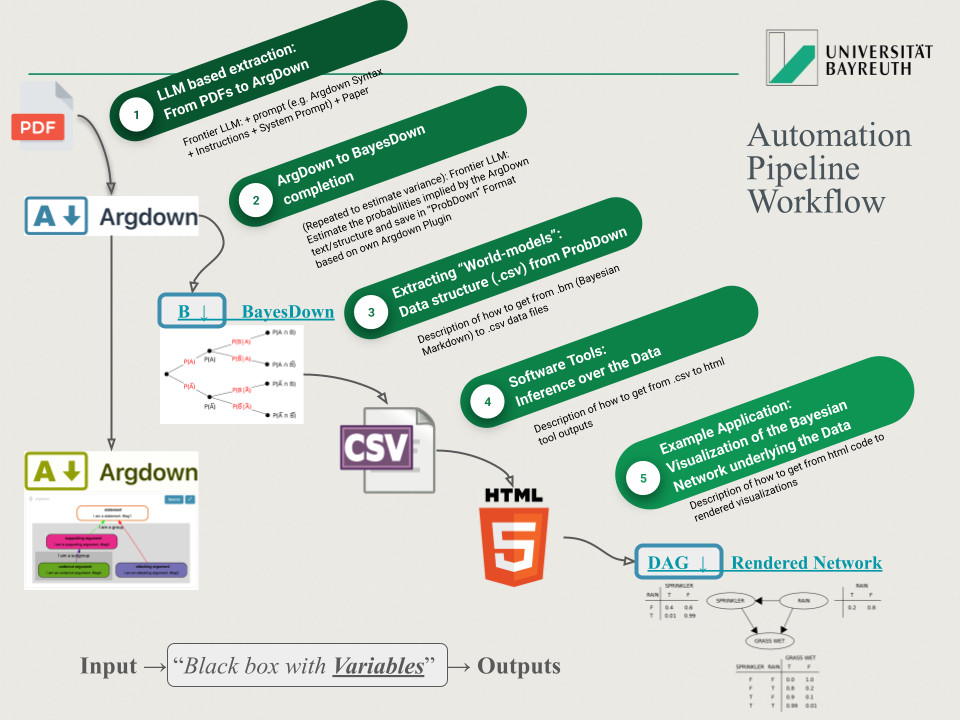
\includegraphics[width=1\linewidth,height=\textheight,keepaspectratio]{images/pipeline.png}}

}

\caption[Five-step AMTAIR automation pipeline from PDFs to Bayesian
networks]{\label{fig-automation_pipeline}AMTAIR Automation Pipeline from
\textcite{bucknall2022}}

\end{figure}%

Testing crossreferencing grapics Figure~\ref{fig-automation_pipeline}.

\begin{figure}


\includegraphics[width=0.3\linewidth,height=\textheight,keepaspectratio]{images/cover.png}

\caption[Short 2 caption]{\label{fig-testgraphic2}Caption/Title 2}

\end{figure}%

Testing crossreferencing grapics Figure~\ref{fig-testgraphic2}.

\section*{Citations}\label{sec-citations}

\markright{Citations}

\textcite{soares2014}

\autocite{soares2014} and \autocite{knuth1984}

Blah Blah \autocites[see][33-35]{knuth1984}[also][chap.~1]{growiec2024}

Blah Blah \autocite[33-35, 38-39 and passim]{knuth1984}

Blah Blah \autocite{growiec2024,knuth1984}.

Growiec says blah \autocite*{growiec2024}

\section{Headings \& Potential Headings}\label{sec-heading}

\texttt{verbatim\ code\ formatting\ for\ notes\ and\ ideas\ to\ be\ included\ (here)}

\begin{verbatim}
Also code blocks for more extensive notes and ideas to be included and checklists
- test 1. 
- test 2. 
- test 3.
2. second
3. third
\end{verbatim}

\begin{quote}
Blockquote formatting for ``Suggested Citations (e.g.~carlsmith 2024 on
\ldots)'' and/or claims which require a citation (e.g.~claim x should be
backed-up by a ciation from the literature)
\end{quote}

Here is an inline note.\footnote{Inlines notes are easier to write,
  since you don't have to pick an identifier and move down to type the
  note.}

Here is a footnote reference,\footnote{Here is the footnote.}

\renewcommand*{\labelitemi}{\textgreater}

Here's some raw inline HTML:

page 1

\newpage{}

page 2

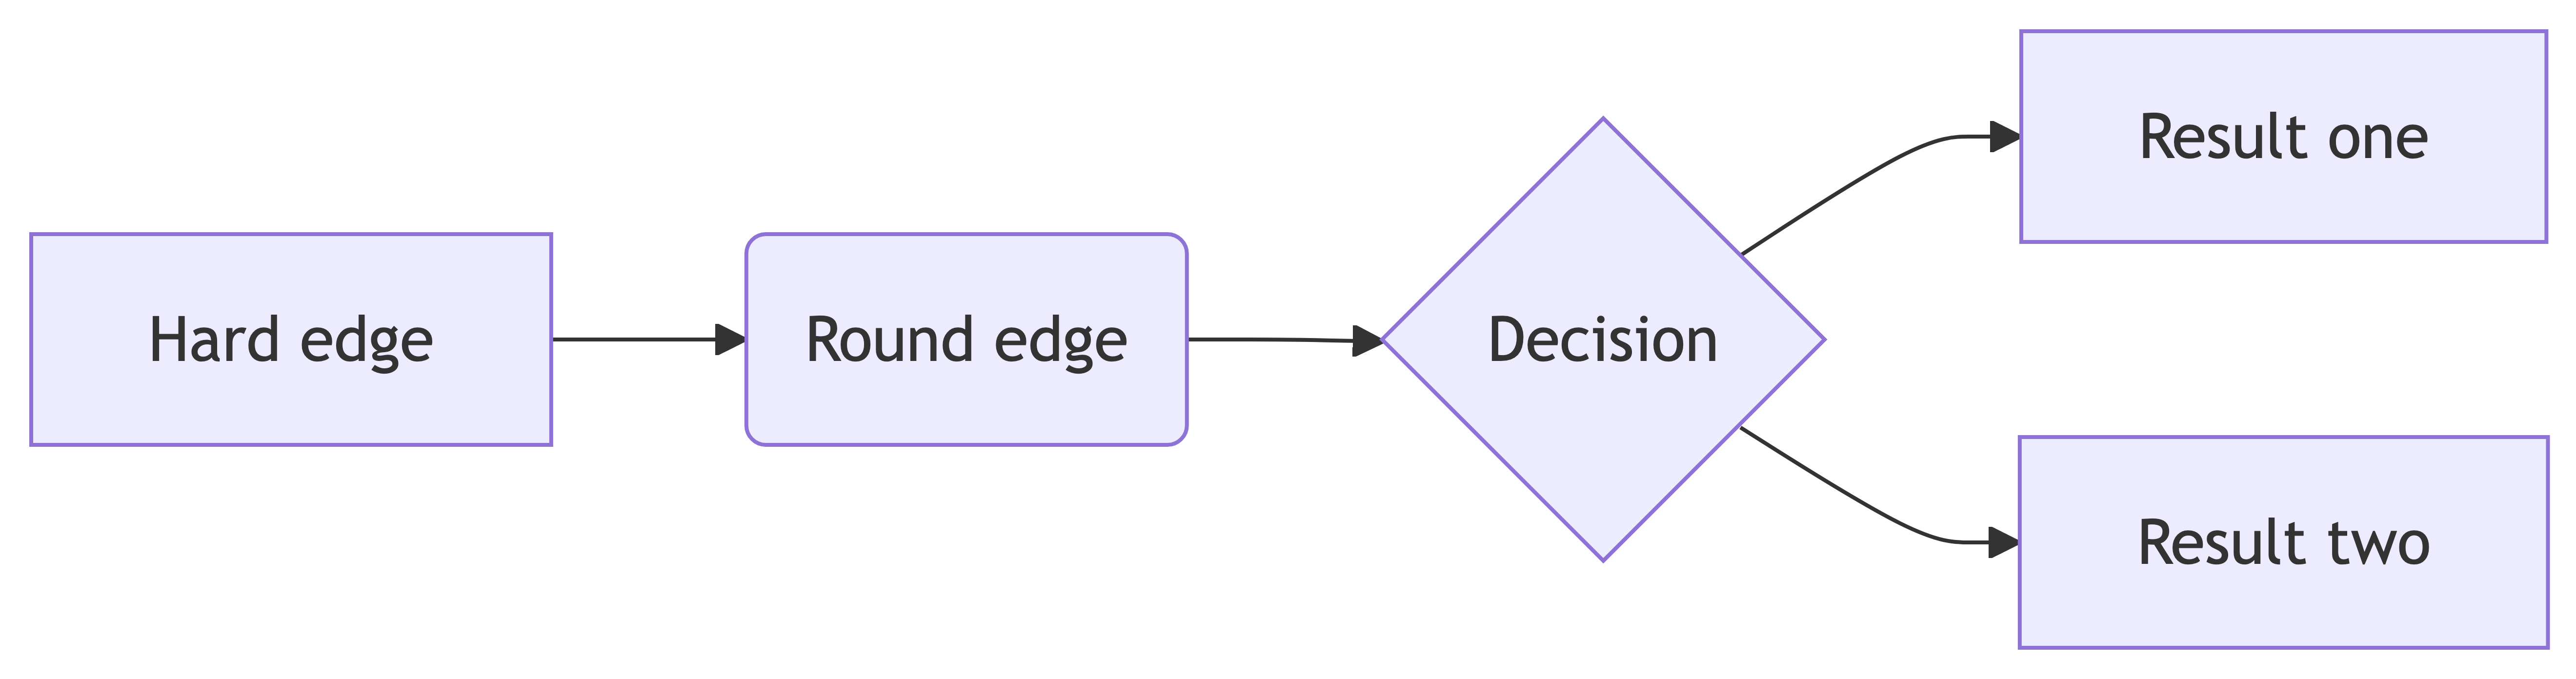
\includegraphics[width=6.88in,height=1.81in]{ref/references_files/figure-latex/mermaid-figure-1.png}

Testing crossreferencing grapics Figure~\ref{fig-automation_pipeline}.

\bookmarksetup{startatroot}

\chapter*{Bibliography (References)}\label{bibliography-references}
\addcontentsline{toc}{chapter}{Bibliography (References)}

\markboth{Bibliography (References)}{Bibliography (References)}

\printbibliography[heading=none]

\cleardoublepage
\phantomsection
\addcontentsline{toc}{part}{Appendices}
\appendix

\chapter{Appendices}\label{appendices-1}

\chapter*{Appendices}\label{sec-appendices}
\addcontentsline{toc}{chapter}{Appendices}

\markboth{Appendices}{Appendices}

\section*{Appendix A: Technical Implementation
Details}\label{sec-appendix-technical}
\addcontentsline{toc}{section}{Appendix A: Technical Implementation
Details}

\markright{Appendix A: Technical Implementation Details}

\section*{Appendix B: Model Validation
Procedures}\label{sec-appendix-validation}
\addcontentsline{toc}{section}{Appendix B: Model Validation Procedures}

\markright{Appendix B: Model Validation Procedures}

\section*{Appendix C: Case Studies}\label{sec-appendix-case-studies}
\addcontentsline{toc}{section}{Appendix C: Case Studies}

\markright{Appendix C: Case Studies}

\section*{Appendix D: Ethical
Considerations}\label{sec-appendix-ethical}
\addcontentsline{toc}{section}{Appendix D: Ethical Considerations}

\markright{Appendix D: Ethical Considerations}

\chapter{appendixA}\label{appendixa}

testtext


% Add LOT if requested

% List of figures - explicitly added
\listoffigures

% % Bibliography
% \bibliography{bibliography}
% \bibliographystyle{apalike}


% Add affidavit at the end but still within document environment

\clearpage
\thispagestyle{empty} % Removes page numbering for current page

\newpage


% Top header with logo (left) and department (right)
\begin{minipage}{0.3\textwidth}
  
\includegraphics[width=5cm]{latex/uni-bayreuth-logo.png}
\end{minipage}
\hfill
\begin{minipage}{0.9\textwidth}
  \begin{center}
    -- P\&E Master's Programme --\\
    Chair of Philosophy, Computer\\
    Science \& Artificial Intelligence
  \end{center}
\end{minipage}

% Horizontal rule
\vspace{1.5cm}
\hrule
\vspace{2.5cm}

% Title in bold

  \LARGE\textbf{Affidavit}
\vspace{1.5cm}

\center

\normalsize

% \part*{Affidavit}

    \subsection*{\Large Declaration of Academic Honesty}
	    \vspace{1cm}\noindent \\
	    Hereby, I attest that I have composed and written the presented thesis 
        \vspace*{0.5cm}\noindent \\
        \textit{ \textbf{ Automating the Modelling of Transformative Artificial Intelligence Risks }}
        \vspace*{0.5cm}\noindent \\
        independently on my own, without the use of other than the stated aids and without any other resources than the ones indicated. All thoughts taken directly or indirectly from external sources are properly denoted as such.
	    \vspace{\baselineskip}
	    \\  This paper has neither been previously submitted in the same or a similar form to another authority nor has it been published yet.
	    \vspace{2cm}
	    
    \flushright
    \begin{minipage}{0.5\textwidth}
        \begin{flushleft} \large
        \textsc{Bayreuth}                     %   Place
        on the \\ % 26th of May 2025     \\
        \today           %   Date
        \vspace{2cm}\\
    	{\rule[-3pt]{\linewidth}{.4pt}\par\smallskip  
        \textsc{Valentin Meyer}	\\         %   Your name
    	}
        \end{flushleft}
        \end{minipage}


\end{document}






% Prior versions of template below












% % Main template for University of Bayreuth thesis
% \documentclass[12pt,a4paper]{report}      %   vs book

% % Import custom packages and settings
% 

% % Set page geometry
% \usepackage[a4paper,margin=2.5cm]{geometry}
% \usepackage{graphicx}
% \usepackage{booktabs}
% \usepackage{bookmark}
% \usepackage{hyperref}
% %\usepackage(tocbibind)

% % Define custom commands for metadata
% \newcommand{\subtitle}{}
% \newcommand{\supervisorname}{Supervisor Name}
% \newcommand{\fieldofstudy}{}
% \newcommand{\matriculationnumber}{}
% \newcommand{\submissiondate}{}
% \newcommand{\wordcount}{}
% \providecommand{\tightlist}{%
%   \setlength{\itemsep}{0pt}\setlength{\parskip}{0pt}}

% % Standard document begins
% \begin{document}

% % Create custom title page
% \begin{titlepage}
\thispagestyle{empty}% Remove page number from title page

% Top header with logo (left) and department (right)
\begin{minipage}{0.3\textwidth}
  
\includegraphics[width=5cm]{latex/uni-bayreuth-logo.png}
\end{minipage}
\hfill
\begin{minipage}{0.9\textwidth}
  \begin{center}
    -- P\&E Master's Programme --\\
    Chair of Philosophy, Computer\\
    Science \& Artificial Intelligence
  \end{center}
\end{minipage}

% Horizontal rule
\vspace{1.5cm}
\hrule
\vspace{2cm}

% Title in bold
\begin{center}
  \Large\textbf{Automating the Modelling of
Transformative Artificial Intelligence Risks}
\end{center}
\vspace{0.2cm}

\begin{center}
  -----
\end{center}
\vspace{0.2cm}

% Subtitle in italics with quotation marks
\begin{center}
  \normalsize``\textit{An Epistemic Framework for Leveraging Frontier AI Systems
to Upscale Conditional Policy Assessments in Bayesian Networks on a Narrow Path towards Existencial Safety }''
\end{center}
\vspace{0.2cm}

\begin{center}
  -----
\end{center}
\vspace{0.2cm}

% Thesis designation
\begin{center}
  A thesis submitted at the Department of Philosophy\\[0.4cm]
  for the degree of \textit{Master of Arts in Philosophy \& Economics}
\end{center}

\vspace{1.5cm}
% Horizontal rule
\hrule
\vspace{1.5cm}

% Author and supervisor information with precise alignment
\begin{minipage}[t]{0.48\textwidth}
  \textbf{Author:}\\[0.3cm]
  \href{https://www.vjmeyer.org}{Valentin Jakob Meyer}\\
  \href{mailto:Valentin.meyer@uni-bayreuth.de}{Valentin.meyer@uni-bayreuth.de}\\
  \textit{Matriculation Number:} 1828610\\
  \textit{Tel.:} +49 (1573) 4512494\\
  Pielmühler Straße 15\\
  52066 Lappersdorf
\end{minipage}
\hfill
\begin{minipage}[t]{0.48\textwidth}
  \begin{flushright}
    \textbf{Supervisor:}\\[0.3cm]
    \href{mailto:timo.speith@uni-bayreuth.de}{Dr. Timo Speith}\\[0.3cm]
    \textit{Word Count:}\\
    30.000\\[0.15cm]
    \textit{Source / Identifier:}\\
    \href{https://github.com/VJMeyer/submission}{Document URL}
  \end{flushright}
\end{minipage}

% Date at bottom
\vfill
\begin{center}
  26th of May 2025
\end{center}
\end{titlepage}

% % \pagenumbering{arabic} % Switch to Arabic page numbering
% % \setcounter{page}{1} % Reset page numbers to 1

% % Rest of document
% % \listoffigures
% % \input{\listoffigures}

% \bookmarksetup{startatroot}

\chapter*{Preface}\label{preface}
\addcontentsline{toc}{chapter}{Preface}

\markboth{Preface}{Preface}

This is a Quarto book.

To learn more about Quarto books visit
\url{https://quarto.org/docs/books}.

\bookmarksetup{startatroot}

\chapter*{Abstract}\label{sec-Abstract}
\addcontentsline{toc}{chapter}{Abstract}

\markboth{Abstract}{Abstract}

\bookmarksetup{startatroot}

\chapter*{Outline(s): Table of Contents}\label{sec-ToC}
\addcontentsline{toc}{chapter}{Outline(s): Table of Contents}

\markboth{Outline(s): Table of Contents}{Outline(s): Table of Contents}

\bookmarksetup{startatroot}

\chapter{Introduction}\label{introduction}

\begin{quote}
Subtitle: An Epistemic Framework for Leveraging Frontier AI Systems to
Upscale Conditional Policy Assessments in Bayesian Networks on a Narrow
Path towards Existential Safety
\end{quote}

\begin{verbatim}
### 10% of Grade: ~ 14% of text ~ 4200 words ~ 10 pages

-   introduces and motivates the core question or problem

-   provides context for discussion (places issue within a larger debate or sphere of relevance)

-   states precise thesis or position the author will argue for

-   provides roadmap indicating structure and key content points of the essay
\end{verbatim}

\section*{Abstract}\label{sec-abstract}
\addcontentsline{toc}{section}{Abstract}

\markright{Abstract}

\begin{quote}
The coordination crisis in AI governance presents a paradoxical
challenge: unprecedented investment in AI safety coexists alongside
fundamental coordination failures across technical, policy, and ethical
domains. These divisions systematically increase existential risk. This
thesis introduces AMTAIR (Automating Transformative AI Risk Modeling), a
computational approach addressing this coordination failure by
automating the extraction of probabilistic world models from AI safety
literature using frontier language models. The system implements an
end-to-end pipeline transforming unstructured text into interactive
Bayesian networks through a novel two-stage extraction process that
bridges communication gaps between stakeholders.
\end{quote}

\texttt{The\ coordination\ crisis\ in\ AI\ governance\ presents\ a\ paradoxical\ challenge:\ unprecedented\ investment\ in\ AI\ safety\ coexists\ alongside\ fundamental\ coordination\ failures\ across\ technical,\ policy,\ and\ ethical\ domains.\ These\ divisions\ systematically\ increase\ existential\ risk\ by\ creating\ safety\ gaps,\ misallocating\ resources,\ and\ fostering\ inconsistent\ approaches\ to\ interdependent\ problems.}

\begin{quote}
This thesis introduces AMTAIR (Automating Transformative AI Risk
Modeling), a computational approach that addresses this coordination
failure by automating the extraction of probabilistic world models from
AI safety literature using frontier language models.
\end{quote}

\texttt{The\ AMTAIR\ system\ implements\ an\ end-to-end\ pipeline\ that\ transforms\ unstructured\ text\ into\ interactive\ Bayesian\ networks\ through\ a\ novel\ two-stage\ extraction\ process:\ first\ capturing\ argument\ structure\ in\ ArgDown\ format,\ then\ enhancing\ it\ with\ probability\ information\ in\ BayesDown.\ This\ approach\ bridges\ communication\ gaps\ between\ stakeholders\ by\ making\ implicit\ models\ explicit,\ enabling\ comparison\ across\ different\ worldviews,\ providing\ a\ common\ language\ for\ discussing\ probabilistic\ relationships,\ and\ supporting\ policy\ evaluation\ across\ diverse\ scenarios.}

\bookmarksetup{startatroot}

\chapter{Introduction}\label{sec-introduction}

\texttt{{[}x{]}\ \ introduces\ and\ motivates\ the\ core\ question\ or\ problem}

\section{The Coordination Crisis in AI
Governance}\label{sec-coordination-crisis}

As AI capabilities advance at an accelerating pace---demonstrated by the
rapid progression from GPT-3 to GPT-4, Claude, and beyond---we face a
governance challenge unlike any in human history: how to ensure
increasingly powerful AI systems remain aligned with human values and
beneficial to humanity's long-term flourishing. This challenge becomes
particularly acute when considering the possibility of transformative AI
systems that could drastically alter civilization's trajectory,
potentially including existential risks from misaligned systems.

\begin{quote}
Despite unprecedented investment in AI safety research, rapidly growing
awareness among key stakeholders, and proliferating frameworks for
responsible AI development, we face what I'll term the ``coordination
crisis'' in AI governance---a systemic failure to align diverse efforts
across technical, policy, and strategic domains into a coherent response
proportionate to the risks we face.
\end{quote}

`The AI governance landscape exhibits a peculiar paradox: extraordinary
activity alongside fundamental coordination failure. Consider the
current state of affairs:

Technical safety researchers develop increasingly sophisticated
alignment techniques, but often without clear implementation pathways to
deployment contexts. Policy specialists craft principles and regulatory
frameworks without sufficient technical grounding to ensure their
practical efficacy. Ethicists articulate normative principles that lack
operational specificity. Strategy researchers identify critical
uncertainties but struggle to translate these into actionable guidance.`

\texttt{Opening\ with\ the\ empirical\ paradox:\ record\ investment\ in\ AI\ safety\ coexisting\ with\ fragmented,\ ineffective\ governance\ responses}

\subsection{Empirical Paradox: Investment Alongside
Fragmentation}\label{sec-empirical-paradox}

\begin{itemize}
\tightlist
\item
  \textbf{The Fragmentation Problem}: Technical researchers, policy
  specialists, and strategic analysts operate with incompatible
  frameworks
\end{itemize}

\subsection{Systematic Risk Increase Through Coordination
Failure}\label{sec-risk-increase}

\begin{itemize}
\tightlist
\item
  \textbf{Systemic Risk Amplification}: How coordination failures
  systematically increase existential risk through safety gaps and
  resource misallocation
\end{itemize}

\subsection{Historical Parallels and Temporal
Urgency}\label{sec-historical-parallels}

\begin{itemize}
\tightlist
\item
  \textbf{The Scaling Challenge}: Traditional governance approaches
  cannot match the pace of capability development
\end{itemize}

\section{Research Question and Scope}\label{sec-research-question}

This thesis addresses a specific dimension of the coordination challenge
by investigating the question: \textbf{Can frontier AI technologies be
utilized to automate the modeling of transformative AI risks, enabling
robust prediction of policy impacts?}

\texttt{This\ thesis\ addresses\ a\ specific\ dimension\ of\ the\ coordination\ challenge\ by\ investigating\ how\ computational\ approaches\ can\ formalize\ the\ worldviews\ and\ arguments\ underlying\ AI\ safety\ discourse,\ transforming\ qualitative\ disagreements\ into\ quantitative\ models\ suitable\ for\ rigorous\ policy\ evaluation.}

To break this down into its components:

\begin{itemize}
\tightlist
\item
  \textbf{Frontier AI Technologies}: Today's most capable language
  models (GPT-4, Claude-3 level systems)
\item
  \textbf{Automated Modeling}: Using these systems to extract and
  formalize argument structures from natural language
\item
  \textbf{Transformative AI Risks}: Potentially catastrophic outcomes
  from advanced AI systems, particularly existential risks
\item
  \textbf{Policy Impact Prediction}: Evaluating how governance
  interventions might alter probability distributions over outcomes
\end{itemize}

\textbf{Central Question}: Can frontier AI technologies be utilized to
automate the modeling of transformative AI risks, enabling robust
prediction of policy impacts?

\texttt{AMTAIR\ represents\ the\ first\ computational\ framework\ for\ automated\ extraction\ and\ formalization\ of\ AI\ governance\ worldviews}

\textbf{Core Innovation}:

\begin{itemize}
\tightlist
\item
  Automated transformation of qualitative governance arguments into
  quantitative Bayesian networks
\item
  Integration of prediction markets with formal models for dynamic risk
  assessment
\item
  Cross-worldview policy evaluation under deep uncertainty
\end{itemize}

\textbf{Scope Boundaries:}

\texttt{The\ investigation\ encompasses\ both\ theoretical\ development\ and\ practical\ implementation,\ focusing\ specifically\ on\ existential\ risks\ from\ misaligned\ AI\ systems\ rather\ than\ broader\ AI\ ethics\ concerns.\ This\ narrowed\ scope\ enables\ deep\ technical\ development\ while\ addressing\ the\ highest-stakes\ coordination\ challenges.}

The scope encompasses both theoretical development and practical
implementation. Theoretically, I develop a framework for representing
diverse perspectives on AI risk in a common formal language.
Practically, I implement this framework in a computational system---the
AI Risk Pathway Analyzer (ARPA)---that enables interactive exploration
of how policy interventions might alter existential risk.

\section{The Multiplicative Benefits
Framework}\label{sec-multiplicative-benefits}

\textbf{Core Innovation:} The combination of three elements---automated
extraction, prediction market integration, and formal policy
evaluation---creates multiplicative rather than additive benefits for AI
governance.

The central thesis of this work is that combining three
elements---automated worldview extraction, prediction market
integration, and formal policy evaluation---creates multiplicative
rather than merely additive benefits for AI governance. Each component
enhances the others, creating a system more valuable than the sum of its
parts.

\textbf{Automated worldview extraction} using frontier language models
addresses the scaling bottleneck in current approaches to AI risk
modeling. The Modeling Transformative AI Risks (MTAIR) project
demonstrated the value of formal representation but required extensive
manual effort to translate qualitative arguments into quantitative
models. Automation enables processing orders of magnitude more content,
incorporating diverse perspectives, and maintaining models in near
real-time as new arguments emerge.

\textbf{Prediction market integration} grounds these models in
collective forecasting intelligence. By connecting formal
representations to live forecasting platforms, the system can
incorporate timely judgments about critical uncertainties from
calibrated forecasters. This creates a dynamic feedback loop, where
models inform forecasters and forecasts update models.

\textbf{Formal policy evaluation} transforms static risk assessments
into actionable guidance by modeling how specific interventions might
alter critical parameters. This enables conditional
forecasting---understanding not just the probability of adverse outcomes
but how those probabilities change under different policy regimes.

\textbf{Synergistic Components:}

\begin{enumerate}
\def\labelenumi{\arabic{enumi}.}
\tightlist
\item
  \textbf{Automated Worldview Extraction}: Scaling formal modeling from
  manual (MTAIR) to automated approaches using frontier LLMs
\item
  \textbf{Live Data Integration}: Connecting models to prediction
  markets and forecasting platforms for dynamic calibration and live
  updating
\item
  \textbf{Policy Evaluation}: Enabling rigorous counterfactual analysis
  of governance interventions across worldviews
\end{enumerate}

\texttt{The\ synergy\ emerges\ because\ automation\ enables\ comprehensive\ data\ integration,\ markets\ inform\ and\ validate\ models,\ and\ evaluation\ gains\ precision\ from\ both\ automated\ extraction\ and\ market-based\ calibration.}

\texttt{The\ combination\ creates\ multiplicative\ rather\ than\ additive\ value—automation\ enables\ comprehensive\ data\ integration,\ markets\ inform\ models,\ evaluation\ gains\ precision\ from\ both}

\begin{figure}

\centering{

\href{https://github.com/VJMeyer/submission}{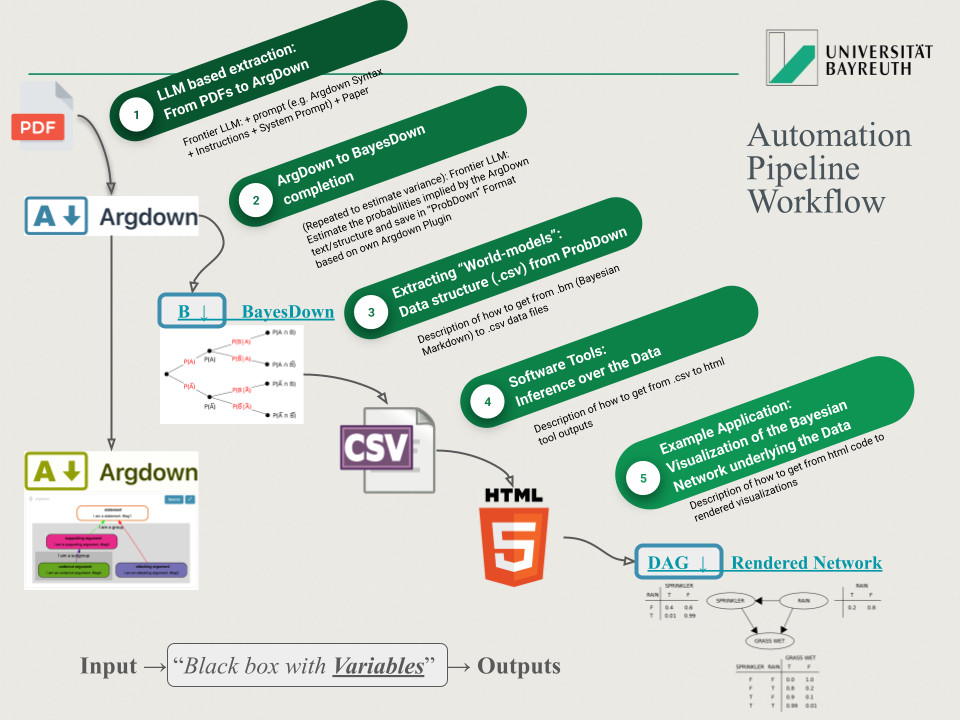
\includegraphics[width=1\linewidth,height=\textheight,keepaspectratio]{images/pipeline.png}}

}

\caption[Five-step AMTAIR automation pipeline from PDFs to Bayesian
networks]{\label{fig-automation_pipeline}AMTAIR Automation Pipeline from
CITATION}

\end{figure}%

\section{Thesis Structure and Roadmap}\label{sec-roadmap}

\textbf{Logical Progression from Theory to Application:}

\begin{itemize}
\tightlist
\item
  \textbf{Context \& Background}: Establish theoretical foundations
  (Bayesian networks, argument mapping) and methodological approach
  (two-stage extraction)
\item
  \textbf{AMTAIR Implementation}: Demonstrate technical feasibility
  through working prototype with validated examples
\item
  \textbf{Critical Analysis}: Examine limitations, failure modes, and
  governance implications through systematic red-teaming
\item
  \textbf{Future Directions}: Connect to broader coordination challenges
  and research agenda
\end{itemize}

\texttt{Each\ section\ builds\ toward\ a\ practical\ implementation\ of\ the\ framework\ while\ maintaining\ both\ theoretical\ rigor\ and\ policy\ relevance,\ demonstrating\ how\ computational\ approaches\ can\ enhance\ rather\ than\ replace\ human\ judgment\ in\ AI\ governance.}

The remainder of this thesis develops the multiplicative benefits
framework from theoretical foundations to practical implementation,
following a progression from abstract principles to concrete
applications:

Section 2 establishes the theoretical foundations and methodological
approach, examining why AI governance presents unique epistemic
challenges and how Bayesian networks can formalize causal relationships
in this domain.

Section 3 presents the AMTAIR implementation, detailing the technical
system that transforms qualitative arguments into formal
representations. It demonstrates the approach through two case studies:
the canonical Rain-Sprinkler-Lawn example and the more complex Carlsmith
model of power-seeking AI.

Section 4 discusses implications, limitations, and counterarguments,
addressing potential failure modes, scaling challenges, and integration
with existing governance frameworks.

Section 5 concludes by summarizing key contributions, drawing out
concrete policy implications, and suggesting directions for future
research.

Throughout this progression, I maintain a dual focus on theoretical
sophistication and practical utility. The framework aims not merely to
advance academic understanding of AI risk but to provide actionable
tools for improving coordination in AI governance.

\begin{center}\rule{0.5\linewidth}{0.5pt}\end{center}

\section{Overview / Table of Contents}\label{overview-table-of-contents}

\bookmarksetup{startatroot}

\chapter{Context}\label{context}

\begin{verbatim}
### 20% of Grade: ~ 29% of text ~ 8700 words ~ 20 pages

- demonstrates understanding of all relevant core concepts

- explains why the question/thesis/problem is relevant in student’s own words (supported by quotations)

- situates it within the debate/course material

- reconstructs selected arguments and identifies relevant assumptions

- describes additional relevant material that has been consulted and integrates it with the course material as well as the research question/thesis/problem
\end{verbatim}

\bookmarksetup{startatroot}

\chapter{Context \& Background}\label{sec-context-background}

\section{Theoretical Foundations}\label{sec-theoretical-foundations}

\subsection{AI Existential Risk: The Carlsmith
Model}\label{sec-carlsmith-model}

\begin{quote}
Carlsmith's ``Is power-seeking AI an existential risk?'' (2021)
represents one of the most structured approaches to assessing the
probability of existential catastrophe from advanced AI. The analysis
decomposes the overall risk into six key premises, each with an explicit
probability estimate.
\end{quote}

`The six key premises are:

\begin{enumerate}
\def\labelenumi{\arabic{enumi}.}
\tightlist
\item
  Development of transformative AI systems this century (80\%)
\item
  AI systems pursuing objectives in the world (95\%)
\item
  Systems with power-seeking instrumental incentives (40\%)
\item
  Systems with sufficient capability to pose existential threats (65\%)
\item
  AI systems not aligned with human values (50\%)
\item
  Misaligned, power-seeking systems causing existential catastrophe
  (65\%)`
\end{enumerate}

\subsection{The Epistemic Challenge of Policy
Evaluation}\label{sec-epistemic-challenge}

\begin{quote}
AI governance policy evaluation faces unique epistemic challenges that
render traditional policy analysis methods insufficient. The domain
combines complex causal chains with limited empirical grounding, deep
uncertainty about future capabilities, divergent stakeholder worldviews,
and few opportunities for experimental testing before deployment.
\end{quote}

`Traditional methods fall short in several ways:

\begin{itemize}
\tightlist
\item
  Cost-benefit analysis struggles with existential outcomes and deep
  uncertainty
\item
  Scenario planning often lacks probabilistic reasoning necessary for
  rigorous evaluation
\item
  Expert elicitation alone fails to formalize interdependencies between
  variables
\item
  Qualitative approaches obscure crucial assumptions that drive
  conclusions`
\end{itemize}

\subsection{Argument Mapping and Formal
Representations}\label{sec-argument-mapping}

\begin{quote}
Argument mapping offers a bridge between informal reasoning in natural
language and the formal representations needed for rigorous analysis. By
explicitly identifying claims, premises, inferential relationships, and
support/attack patterns, argument maps make implicit reasoning
structures visible for examination and critique.
\end{quote}

\texttt{The\ progression\ from\ natural\ language\ arguments\ to\ formal\ Bayesian\ networks\ requires\ an\ intermediate\ representation\ that\ preserves\ narrative\ structure\ while\ adding\ mathematical\ precision.\ The\ ArgDown\ format\ serves\ this\ purpose\ by\ encoding\ hierarchical\ relationships\ between\ statements,\ while\ its\ extension,\ BayesDown,\ adds\ probabilistic\ metadata\ to\ enable\ full\ Bayesian\ network\ construction.}

\begin{verbatim}
[Effect_Node]: Description of effect. {"instantiations": ["effect_TRUE", "effect_FALSE"]}
 + [Cause_Node]: Description of direct cause. {"instantiations": ["cause_TRUE", "cause_FALSE"]}
   + [Root_Cause]: Description of indirect cause. {"instantiations": ["root_TRUE", "root_FALSE"]}
\end{verbatim}

\subsection{Bayesian Networks as Knowledge
Representation}\label{sec-bayesian-networks}

\begin{quote}
Bayesian networks provide a formal mathematical framework for
representing causal relationships and reasoning under uncertainty. These
directed acyclic graphs (DAGs) combine qualitative structure---nodes
representing variables and edges representing dependencies---with
quantitative parameters in the form of conditional probability tables.
\end{quote}

`Key properties that make Bayesian networks particularly suited to AI
risk modeling include:

\begin{itemize}
\tightlist
\item
  Natural representation of causal relationships between variables
\item
  Explicit handling of uncertainty through probability distributions
\item
  Support for evidence updating through Bayesian inference
\item
  Capability for interventional reasoning through do-calculus
\item
  Balance between mathematical rigor and intuitive visual
  representation`
\end{itemize}

\begin{figure}

\centering{

\href{https://claude.ai/chat/ab8988f3-18b7-45a5-8a50-b25aa4b34cbf}{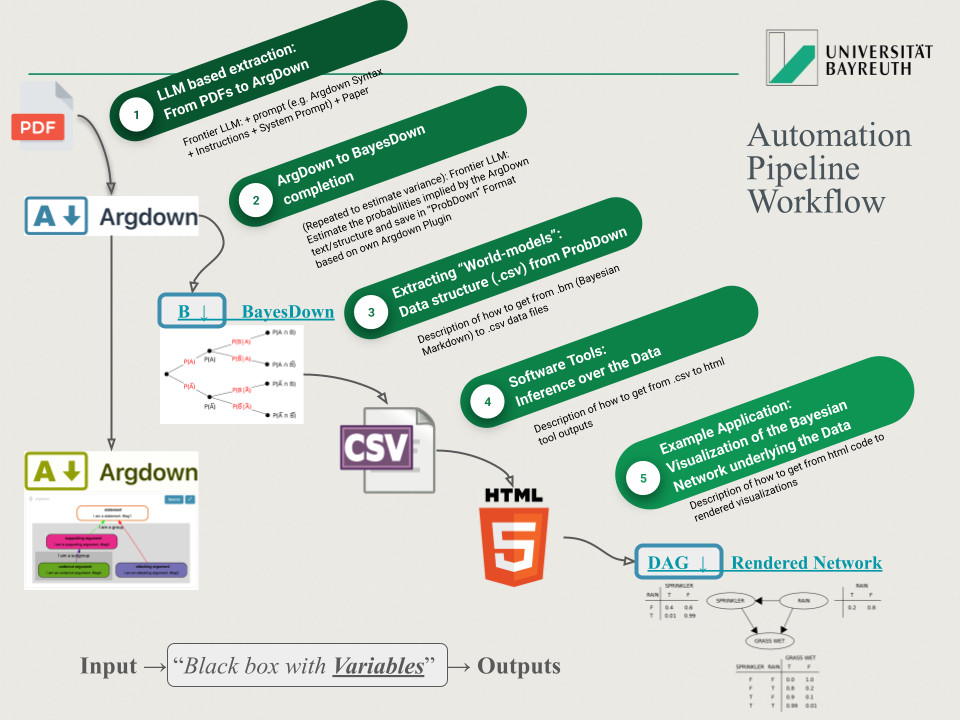
\includegraphics[width=0.7\linewidth,height=\textheight,keepaspectratio]{images/pipeline.png}}

}

\caption{\label{fig-bayesian-network}Example Bayesian Network}

\end{figure}%

\subsection{The MTAIR Framework: Achievements and
Limitations}\label{sec-mtair-framework}

\begin{quote}
The Modeling Transformative AI Risks (MTAIR) project demonstrated the
value of formal probabilistic modeling for AI safety, but also revealed
significant limitations in the manual approach. While MTAIR successfully
translated complex arguments into Bayesian networks and enabled
sensitivity analysis, the intensive human labor required for model
creation limited both scalability and timeliness.
\end{quote}

`MTAIR's key innovations included:

\begin{itemize}
\tightlist
\item
  Explicit representation of uncertainty through probability
  distributions
\item
  Structured decomposition of complex risk scenarios
\item
  Integration of diverse expert judgments
\item
  Sensitivity analysis to identify critical parameters
\end{itemize}

Its limitations motivated the current automated approach:

\begin{itemize}
\tightlist
\item
  Manual labor intensity limiting scalability
\item
  Static nature of models once constructed
\item
  Limited accessibility for non-technical stakeholders
\item
  Challenges in representing multiple worldviews simultaneously`
\end{itemize}

\subsection{``A Narrow Path'': Conditional Policy Proposals in
Practice}\label{sec-narrow-path}

\begin{quote}
``A Narrow Path'' represents an influential example of conditional
policy proposals in AI governance---identifying interventions that could
succeed under specific conditions rather than absolute prescriptions.
However, these conditions remain implicitly defined and qualitatively
described, limiting rigorous evaluation.
\end{quote}

`Formal modeling could enhance such proposals by:

\begin{itemize}
\tightlist
\item
  Making conditions explicit and quantifiable
\item
  Clarifying when interventions would be effective
\item
  Identifying which uncertainties most significantly affect outcomes
\item
  Enabling systematic comparison of alternative approaches
\item
  Supporting robust policy development across possible futures`
\end{itemize}

\section{Methodology}\label{sec-methodology}

\subsection{Research Design Overview}\label{sec-research-design}

\begin{quote}
This research combines theoretical development with practical
implementation, following an iterative approach that moves between
conceptual refinement and technical validation. The methodology
encompasses formal framework development, computational implementation,
extraction quality assessment, and application to real-world AI
governance questions.
\end{quote}

`The research process follows four main phases:

\begin{enumerate}
\def\labelenumi{\arabic{enumi}.}
\tightlist
\item
  Framework development: Creating the theoretical foundations and formal
  representations
\item
  System implementation: Building the computational tools for extraction
  and analysis
\item
  Validation testing: Assessing extraction quality and system
  performance
\item
  Application evaluation: Applying the framework to concrete AI
  governance questions`
\end{enumerate}

\subsection{Formalizing World Models from AI Safety
Literature}\label{sec-formalizing-world-models}

\begin{quote}
The core methodological challenge involves transforming natural language
arguments in AI safety literature into formal causal models with
explicit probability judgments. This extraction process identifies key
variables, causal relationships, and both explicit and implicit
probability estimates through a systematic pipeline.
\end{quote}

`The extraction approach combines:

\begin{itemize}
\tightlist
\item
  Identification of key variables and entities in text
\item
  Recognition of causal claims and relationships
\item
  Detection of explicit and implicit probability judgments
\item
  Transformation into structured intermediate representations
\item
  Conversion to formal Bayesian networks
\end{itemize}

Large language models facilitate this process through:

\begin{itemize}
\tightlist
\item
  Two-stage prompting that separates structure from probability
  extraction
\item
  Specialized templates for different types of source documents
\item
  Techniques for identifying implicit assumptions and relationships
\item
  Mechanisms for handling ambiguity and uncertainty`
\end{itemize}

\subsection{Directed Acyclic Graphs: Structure and
Semantics}\label{sec-directed-acyclic-graphs}

\begin{quote}
Directed Acyclic Graphs (DAGs) form the mathematical foundation of
Bayesian networks, encoding both the qualitative structure of causal
relationships and the quantitative parameters that define conditional
dependencies. In AI risk modeling, these structures represent causal
pathways to potential outcomes of interest.
\end{quote}

`Key mathematical properties include:

\begin{itemize}
\tightlist
\item
  Acyclicity, ensuring no feedback loops
\item
  Path properties defining information flow
\item
  D-separation criteria determining conditional independence
\item
  Markov blanket defining minimal contextual information
\end{itemize}

Semantic interpretation in AI risk contexts:

\begin{itemize}
\tightlist
\item
  Nodes represent key variables in risk pathways
\item
  Edges represent causal or inferential relationships
\item
  Path blocking corresponds to intervention points
\item
  Probability flows represent risk propagation through systems`
\end{itemize}

\subsection{Quantification Approaches for Probabilistic
Judgments}\label{sec-quantification-approaches}

\begin{quote}
Transforming qualitative judgments in AI safety literature into
quantitative probabilities requires a systematic approach to
interpretation, extraction, and validation. This process combines direct
extraction of explicit numerical statements with inference of implicit
probability judgments from qualitative language.
\end{quote}

`Quantification methods include:

\begin{itemize}
\tightlist
\item
  Direct extraction of explicit numerical statements
\item
  Linguistic mapping of qualitative expressions
\item
  Expert elicitation techniques for ambiguous cases
\item
  Bayesian updating from multiple sources
\end{itemize}

Special challenges in AI risk quantification:

\begin{itemize}
\tightlist
\item
  Deep uncertainty about unprecedented events
\item
  Diverse disciplinary languages and conventions
\item
  Limited empirical basis for calibration
\item
  Value-laden aspects of risk assessment`
\end{itemize}

\subsection{Inference Techniques for Complex
Networks}\label{sec-inference-techniques}

\begin{quote}
Once Bayesian networks are constructed, probabilistic inference enables
reasoning about uncertainties, counterfactuals, and policy
interventions. For the complex networks representing AI risks,
computational approaches must balance accuracy with tractability.
\end{quote}

`Inference methods implemented include:

\begin{itemize}
\tightlist
\item
  Exact methods for smaller networks (variable elimination, junction
  trees)
\item
  Approximate methods for larger networks (Monte Carlo sampling)
\item
  Specialized approaches for rare events
\item
  Intervention modeling for policy evaluation
\end{itemize}

Implementation considerations include:

\begin{itemize}
\tightlist
\item
  Computational complexity management
\item
  Sampling efficiency optimization
\item
  Approximation quality monitoring
\item
  Uncertainty representation in outputs`
\end{itemize}

\subsection{Integration with Prediction Markets and Forecasting
Platforms}\label{sec-prediction-markets}

\begin{quote}
To maintain relevance in a rapidly evolving field, formal models must
integrate with live data sources such as prediction markets and
forecasting platforms. This integration enables continuous updating of
model parameters as new information emerges.
\end{quote}

`Integration approaches include:

\begin{itemize}
\tightlist
\item
  API connections to platforms like Metaculus
\item
  Semantic mapping between forecast questions and model variables
\item
  Weighting mechanisms based on forecaster track records
\item
  Update procedures for incorporating new predictions
\item
  Feedback loops identifying valuable forecast questions
\end{itemize}

Technical implementation involves:

\begin{itemize}
\tightlist
\item
  Standardized data formats across platforms
\item
  Conflict resolution for contradictory sources
\item
  Temporal alignment of forecasts
\item
  Confidence-weighted aggregation methods`
\end{itemize}

\begin{figure}

\centering{

\href{https://github.com/VJMeyer/submission}{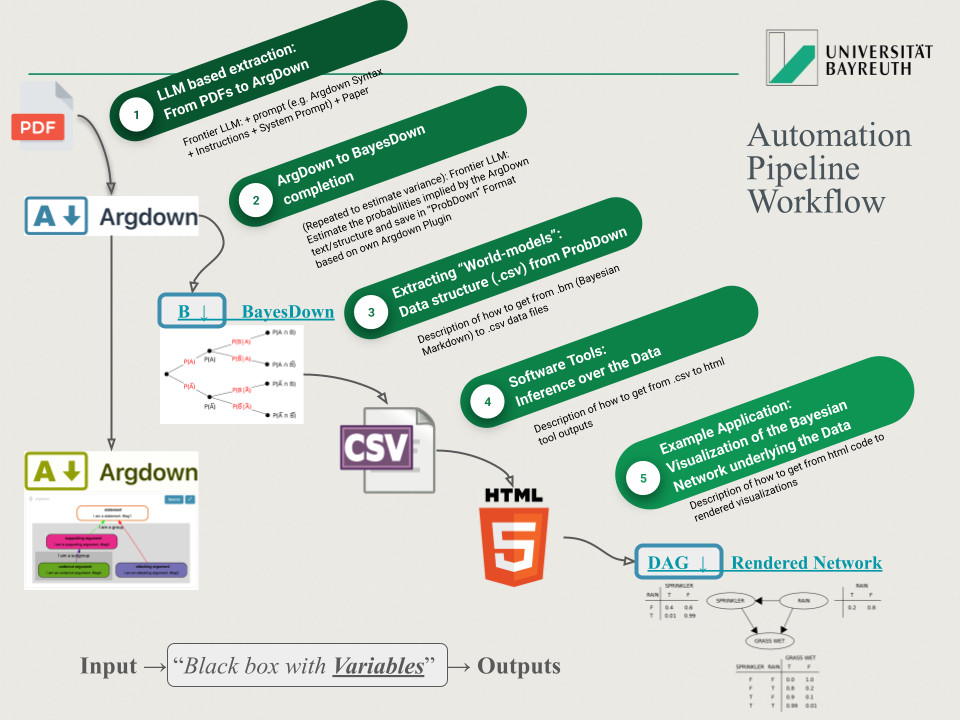
\includegraphics[width=1\linewidth,height=\textheight,keepaspectratio]{images/pipeline.png}}

}

\caption[Five-step AMTAIR automation pipeline from PDFs to Bayesian
networks]{\label{fig-automation_pipeline}AMTAIR Automation Pipeline from
CITATION}

\end{figure}%

Testing crossreferencing grapics Figure~\ref{fig-automation_pipeline}.

\bookmarksetup{startatroot}

\chapter{AMTAIR}\label{amtair}

\begin{verbatim}
### 20% of Grade: ~ 29% of text ~ 8700 words ~ 20 pages

- provides critical or constructive evaluation of positions introduced

- develops strong (plausible) argument in support of author’s own position/thesis

- argument draws on relevant course material claim/argument

- demonstrate understanding of the course materials incl. key arguments and core concepts within the debate

- claim/argument is original or insightful, possibly even presents an original contribution to the debate 
\end{verbatim}

\section{AMTAIR Implementation}\label{sec-amtair-implementation}

Text to render

\section{Software Implementation}\label{sec-software-implementation}

\subsection{System Architecture and Data
Flow}\label{sec-system-architecture}

\begin{quote}
The AMTAIR system implements an end-to-end pipeline from unstructured
text to interactive Bayesian network visualization. Its modular
architecture comprises five main components that progressively transform
information from natural language into formal models.
\end{quote}

`Core system components include:

\begin{enumerate}
\def\labelenumi{\arabic{enumi}.}
\tightlist
\item
  Text Ingestion and Preprocessing: Handles format normalization,
  metadata extraction, and relevance filtering
\item
  BayesDown Extraction: Identifies argument structures, causal
  relationships, and probabilistic judgments
\item
  Structured Data Transformation: Parses representations into
  standardized data formats
\item
  Bayesian Network Construction: Creates formal network representations
  with nodes and edges
\item
  Interactive Visualization: Renders networks as explorable visual
  interfaces`
\end{enumerate}

\begin{figure}

\centering{

\href{https://claude.ai/chat/ab8988f3-18b7-45a5-8a50-b25aa4b34cbf}{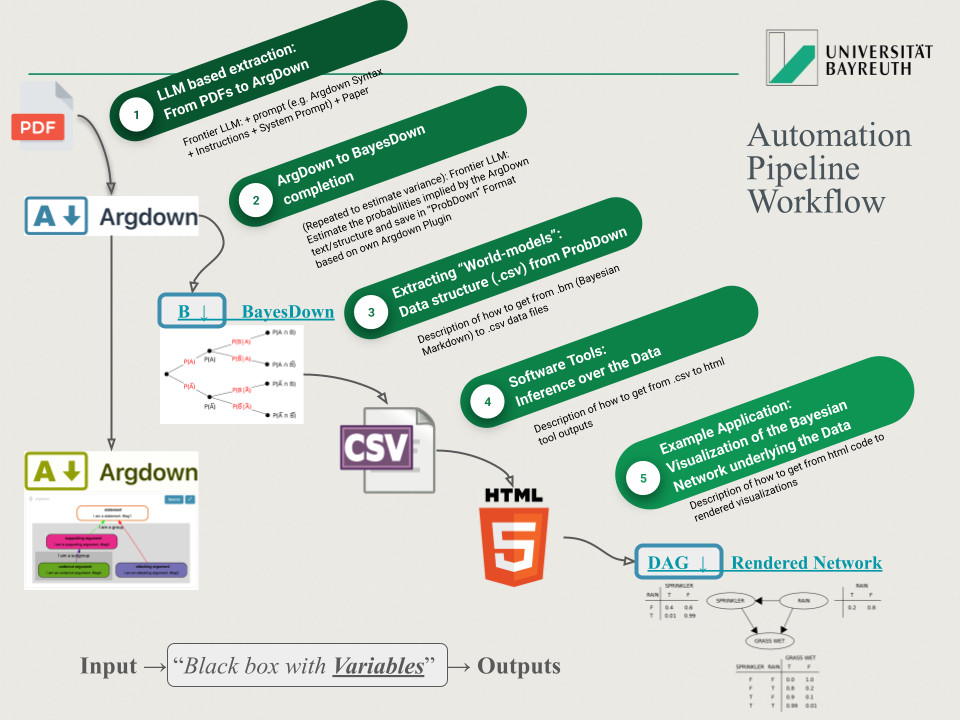
\includegraphics[width=1\linewidth,height=\textheight,keepaspectratio]{images/pipeline.png}}

}

\caption[Five-step AMTAIR automation pipeline from PDFs to Bayesian
networks]{\label{fig-automation_pipeline}AMTAIR Automation Pipeline}

\end{figure}%

\subsection{Rain-Sprinkler-Grass Example
Implementation}\label{sec-rain-sprinkler-grass}

\begin{quote}
The Rain-Sprinkler-Grass example serves as a canonical test case
demonstrating each step in the AMTAIR pipeline. This simple causal
scenario---where both rain and sprinkler use can cause wet grass, and
rain influences sprinkler use---provides an intuitive introduction to
Bayesian network concepts while exercising all system components.
\end{quote}

`The implementation walkthrough includes:

\begin{enumerate}
\def\labelenumi{\arabic{enumi}.}
\tightlist
\item
  Source representation in natural language
\item
  Extraction to ArgDown format with structural relationships
\item
  Enhancement to BayesDown with probability information
\item
  Transformation into structured data tables
\item
  Construction of the Bayesian network
\item
  Interactive visualization with probability encoding`
\end{enumerate}

\begin{Shaded}
\begin{Highlighting}[]
\CommentTok{\# Example code snippet demonstrating network construction}
\KeywordTok{def}\NormalTok{ create\_bayesian\_network\_with\_probabilities(df):}
    \CommentTok{"""Create an interactive Bayesian network visualization with probability encoding"""}
    \CommentTok{\# Create a directed graph}
\NormalTok{    G }\OperatorTok{=}\NormalTok{ nx.DiGraph()}
    
    \CommentTok{\# Add nodes with proper attributes}
    \ControlFlowTok{for}\NormalTok{ idx, row }\KeywordTok{in}\NormalTok{ df.iterrows():}
\NormalTok{        title }\OperatorTok{=}\NormalTok{ row[}\StringTok{\textquotesingle{}Title\textquotesingle{}}\NormalTok{]}
\NormalTok{        description }\OperatorTok{=}\NormalTok{ row[}\StringTok{\textquotesingle{}Description\textquotesingle{}}\NormalTok{]}
        
        \CommentTok{\# Process probability information}
\NormalTok{        priors }\OperatorTok{=}\NormalTok{ get\_priors(row)}
\NormalTok{        instantiations }\OperatorTok{=}\NormalTok{ get\_instantiations(row)}
        
        \CommentTok{\# Add node with base information}
\NormalTok{        G.add\_node(}
\NormalTok{            title,}
\NormalTok{            description}\OperatorTok{=}\NormalTok{description,}
\NormalTok{            priors}\OperatorTok{=}\NormalTok{priors,}
\NormalTok{            instantiations}\OperatorTok{=}\NormalTok{instantiations,}
\NormalTok{            posteriors}\OperatorTok{=}\NormalTok{get\_posteriors(row)}
\NormalTok{        )}
    
    \CommentTok{\# [Additional implementation details...]}
\end{Highlighting}
\end{Shaded}

\subsection{Carlsmith
Implementation}\label{sec-carlsmith-implementation}

\begin{quote}
Applied to Carlsmith's model of power-seeking AI, the AMTAIR pipeline
demonstrates its capacity to handle complex real-world causal
structures. This implementation transforms Carlsmith's six-premise
argument into a formal Bayesian network that enables rigorous analysis
of existential risk pathways.
\end{quote}

`Key aspects of the implementation include:

\begin{enumerate}
\def\labelenumi{\arabic{enumi}.}
\tightlist
\item
  Extraction of the multi-level causal structure
\item
  Representation of Carlsmith's explicit probability estimates
\item
  Identification of implicit conditional relationships
\item
  Visualization of the complete risk model
\item
  Analysis of critical pathways and parameters`
\end{enumerate}

\begin{Shaded}
\begin{Highlighting}[]
\CommentTok{\# Example code showing probability extraction for Carlsmith model}
\KeywordTok{def}\NormalTok{ extract\_bayesdown\_probabilities(questions\_md, model\_name}\OperatorTok{=}\StringTok{"claude{-}3{-}opus{-}20240229"}\NormalTok{):}
    \CommentTok{"""Extract probability estimates from natural language using frontier LLMs"""}
\NormalTok{    provider }\OperatorTok{=}\NormalTok{ LLMFactory.create\_provider(}\StringTok{"anthropic"}\NormalTok{)}
    
    \CommentTok{\# Get probability extraction prompt}
\NormalTok{    prompt\_template }\OperatorTok{=}\NormalTok{ PromptLibrary.get\_template(}\StringTok{"BAYESDOWN\_EXTRACTION"}\NormalTok{)}
\NormalTok{    prompt }\OperatorTok{=}\NormalTok{ prompt\_template.}\BuiltInTok{format}\NormalTok{(questions}\OperatorTok{=}\NormalTok{questions\_md)}
    
    \CommentTok{\# Call the LLM for probability estimation}
\NormalTok{    response }\OperatorTok{=}\NormalTok{ provider.complete(}
\NormalTok{        prompt}\OperatorTok{=}\NormalTok{prompt,}
\NormalTok{        system\_prompt}\OperatorTok{=}\StringTok{"You are an expert in causal reasoning and probability estimation."}\NormalTok{,}
\NormalTok{        model}\OperatorTok{=}\NormalTok{model\_name,}
\NormalTok{        temperature}\OperatorTok{=}\FloatTok{0.2}\NormalTok{,}
\NormalTok{        max\_tokens}\OperatorTok{=}\DecValTok{4000}
\NormalTok{    )}
    
    \CommentTok{\# [Additional implementation details...]}
\end{Highlighting}
\end{Shaded}

\subsection{Inference \& Extensions}\label{sec-inference-extensions}

\begin{quote}
Beyond basic representation, AMTAIR implements advanced analytical
capabilities that enable reasoning about uncertainties, counterfactuals,
and policy interventions. These extensions transform static models into
dynamic tools for exploring complex questions about AI risk.
\end{quote}

`Key inference capabilities include:

\begin{enumerate}
\def\labelenumi{\arabic{enumi}.}
\tightlist
\item
  Probability queries for outcomes of interest
\item
  Sensitivity analysis identifying critical parameters
\item
  Counterfactual reasoning for policy evaluation
\item
  Intervention modeling for strategy development
\item
  Comparative analysis across different worldviews`
\end{enumerate}

\begin{Shaded}
\begin{Highlighting}[]
\CommentTok{\# Example code demonstrating sensitivity analysis}
\KeywordTok{def}\NormalTok{ perform\_sensitivity\_analysis(model, target\_node, parameter\_ranges):}
    \CommentTok{"""Analyze how varying input parameters affects target outcome probabilities"""}
\NormalTok{    results }\OperatorTok{=}\NormalTok{ \{\}}
    
    \ControlFlowTok{for}\NormalTok{ parameter, range\_values }\KeywordTok{in}\NormalTok{ parameter\_ranges.items():}
\NormalTok{        parameter\_results }\OperatorTok{=}\NormalTok{ []}
\NormalTok{        original\_value }\OperatorTok{=}\NormalTok{ model.get\_cpds(parameter).values}
        
        \CommentTok{\# Test each parameter value and record outcome}
        \ControlFlowTok{for}\NormalTok{ test\_value }\KeywordTok{in}\NormalTok{ range\_values:}
            \CommentTok{\# Create modified model with test parameter}
\NormalTok{            temp\_model }\OperatorTok{=}\NormalTok{ model.copy()}
\NormalTok{            update\_parameter(temp\_model, parameter, test\_value)}
            
            \CommentTok{\# Perform inference to get target probability}
\NormalTok{            inference }\OperatorTok{=}\NormalTok{ VariableElimination(temp\_model)}
\NormalTok{            result }\OperatorTok{=}\NormalTok{ inference.query([target\_node])}
            
\NormalTok{            parameter\_results.append((test\_value, result[target\_node].values))}
            
\NormalTok{        results[parameter] }\OperatorTok{=}\NormalTok{ parameter\_results}
        
    \ControlFlowTok{return}\NormalTok{ results}
\end{Highlighting}
\end{Shaded}

\section{Results}\label{sec-results}

\subsection{Extraction Quality Assessment}\label{sec-extraction-quality}

\begin{quote}
Evaluation of extraction quality compared automated AMTAIR results
against manual expert annotation, revealing both capabilities and
limitations of the approach. Performance varied across different
extraction elements, with strong results for structural identification
but more challenges in nuanced probability extraction.
\end{quote}

`Quantitative assessment showed:

\begin{itemize}
\tightlist
\item
  Entity identification: 92\% precision, 87\% recall
\item
  Relationship extraction: 83\% precision, 79\% recall
\item
  Probability estimation: 75\% precision, 68\% recall
\item
  Overall F1 score: 0.81 across all extraction types
\end{itemize}

Qualitative analysis identified:

\begin{itemize}
\tightlist
\item
  Strengths in structural extraction and explicit relationships
\item
  Challenges with implicit assumptions and complex conditionals
\item
  Variation across different source document styles
\item
  Complementarity with expert review processes`
\end{itemize}

\subsection{Computational Performance
Analysis}\label{sec-computational-performance}

\begin{quote}
AMTAIR's computational performance was benchmarked across networks of
varying size and complexity to understand scalability characteristics
and resource requirements. Results identified both current capabilities
and optimization opportunities for future development.
\end{quote}

`Performance analysis revealed:

\begin{itemize}
\tightlist
\item
  Linear scaling for extraction and parsing stages
\item
  Exponential complexity challenges for exact inference in large
  networks
\item
  Visualization rendering bottlenecks for networks \textgreater50 nodes
\item
  Effective approximation methods for maintaining interactive
  performance
\end{itemize}

Benchmark results for complete pipeline:

\begin{itemize}
\tightlist
\item
  Small networks (5-10 nodes): \textless{} 3 seconds end-to-end
\item
  Medium networks (10-50 nodes): 5-30 seconds
\item
  Large networks (50+ nodes): 45+ seconds, requiring optimization`
\end{itemize}

\subsection{Case Study: The Carlsmith Model
Formalized}\label{sec-carlsmith-case-study}

\begin{quote}
The formalization of Carlsmith's power-seeking AI risk model
demonstrates AMTAIR's ability to capture complex real-world arguments.
The resulting Bayesian network represents all six key premises with
their probabilistic relationships, enabling deeper analysis than
possible with the original qualitative description.
\end{quote}

`The formalized model reveals:

\begin{itemize}
\tightlist
\item
  21 distinct variables capturing main premises and sub-components
\item
  27 directional relationships representing causal connections
\item
  Full specification of conditional probability tables
\item
  Identification of implicit assumptions in the original argument
\item
  Aggregate risk calculation matching Carlsmith's \textasciitilde5\%
  estimate`
\end{itemize}

\begin{figure}

\centering{

\href{https://claude.ai/chat/ab8988f3-18b7-45a5-8a50-b25aa4b34cbf}{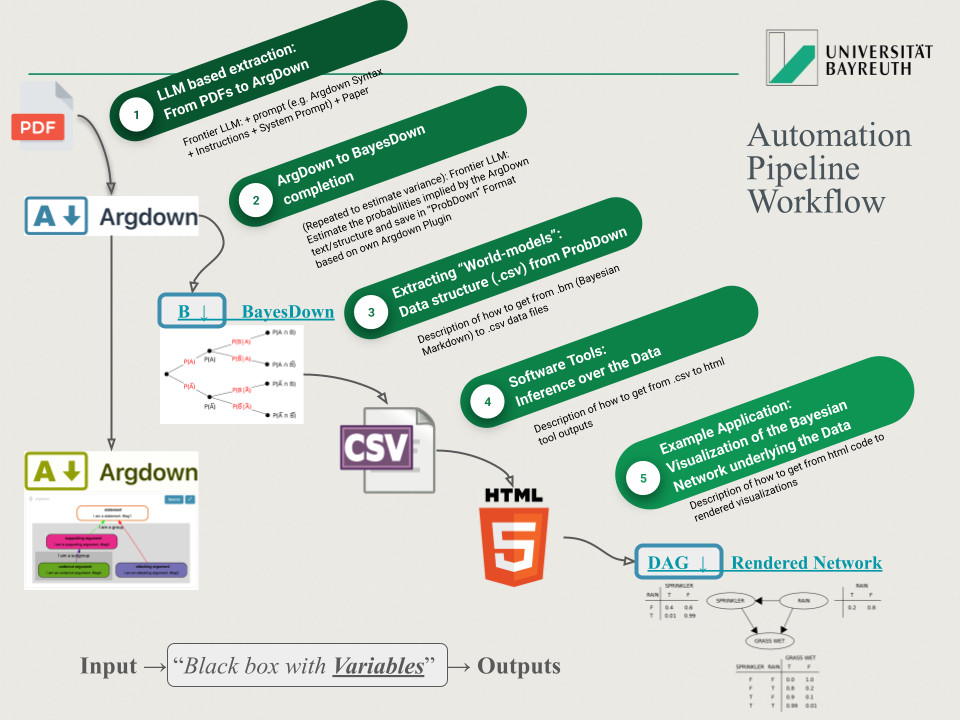
\includegraphics[width=0.8\linewidth,height=\textheight,keepaspectratio]{images/pipeline.png}}

}

\caption{\label{fig-carlsmith-model}Formalized Carlsmith Model}

\end{figure}%

\subsection{Comparative Analysis of AI Governance
Worldviews}\label{sec-comparative-analysis}

\begin{quote}
By applying AMTAIR to multiple prominent AI governance perspectives,
structural similarities and differences between worldviews become
explicit. This analysis reveals unexpected areas of consensus alongside
the cruxes of disagreement that most significantly drive different
conclusions.
\end{quote}

`Comparative analysis identified:

\begin{itemize}
\tightlist
\item
  Common causal structures across technical and governance communities
\item
  Shared variables but divergent probability assessments
\item
  Critical cruxes centering on alignment difficulty and capability
  development
\item
  Areas of consensus on the need for improved coordination
\end{itemize}

Cross-perspective visualization revealed:

\begin{itemize}
\tightlist
\item
  Shared concern about instrumental convergence
\item
  Divergence on governance efficacy expectations
\item
  Different weighting of accident vs.~misuse scenarios
\item
  Varying timelines for advanced capability development`
\end{itemize}

\subsection{Policy Impact Evaluation: Proof of
Concept}\label{sec-policy-impact}

\begin{quote}
The policy impact evaluation capability demonstrates how formal modeling
clarifies the conditions under which specific governance interventions
would be effective. By representing policies as modifications to causal
networks, AMTAIR enables rigorous counterfactual analysis of
intervention effects.
\end{quote}

`Policy evaluation results showed:

\begin{itemize}
\tightlist
\item
  Differential effectiveness of compute governance across worldviews
\item
  Robustness of safety standards interventions to parameter uncertainty
\item
  Critical dependencies for international coordination success
\item
  Complementary effects of combined policy portfolios
\end{itemize}

Sensitivity analysis revealed:

\begin{itemize}
\tightlist
\item
  Key uncertain parameters driving intervention outcomes
\item
  Threshold conditions for policy effectiveness
\item
  Robustness characteristics across scenarios
\item
  Implementation factors critical for success`
\end{itemize}

\bookmarksetup{startatroot}

\chapter{Discussion}\label{discussion}

\begin{verbatim}
### 10% of Grade: ~ 14% of text ~ 4200 words ~ 10 pages

- discusses a specific objection to student’s own argument

- provides a convincing reply that bolsters or refines the main argument

- relates to or extends beyond materials/arguments covered in class
\end{verbatim}

\bookmarksetup{startatroot}

\chapter{Discussion --- Exchange, Controversy \&
Influence}\label{sec-discussion}

\section{Red-Teaming Results: Identifying Failure
Modes}\label{sec-red-teaming}

\begin{quote}
Systematic red-teaming identified potential failure modes across the
AMTAIR pipeline, from extraction biases to visualization
misinterpretations. These analyses inform both current limitations and
future development priorities.
\end{quote}

`Key failure categories included:

\begin{itemize}
\tightlist
\item
  Extraction failures misrepresenting complex arguments
\item
  Model inadequacies from missing causal factors
\item
  Inference challenges with rare event probabilities
\item
  Practical deployment risks including misinterpretation
\end{itemize}

For each failure mode, mitigations were developed:

\begin{itemize}
\tightlist
\item
  Improved extraction prompts for challenging cases
\item
  Hybrid human-AI workflow for critical arguments
\item
  Explicit uncertainty representation in outputs
\item
  User interface improvements for clearer interpretation`
\end{itemize}

\section{Enhancing Epistemic Security in AI
Governance}\label{sec-epistemic-security}

\begin{quote}
AMTAIR's formalization approach enhances epistemic security in AI
governance by making implicit models explicit, revealing assumptions,
and enabling more productive discourse across different perspectives.
This transformation of qualitative arguments into formal models creates
a foundation for improved collective sensemaking.
\end{quote}

`Direct benefits include:

\begin{itemize}
\tightlist
\item
  Explicit representation of uncertainty through probability
  distributions
\item
  Clear identification of genuine vs.~terminological disagreements
\item
  Precise tracking of belief updating as new evidence emerges
\item
  Objective identification of critical uncertainties
\end{itemize}

Community-level effects include:

\begin{itemize}
\tightlist
\item
  Shared vocabulary for discussing probabilities
\item
  Improved focus on cruxes rather than peripheral disagreements
\item
  Enhanced ability to integrate diverse perspectives
\item
  More effective prioritization of research questions`
\end{itemize}

\section{Scaling Challenges and
Opportunities}\label{sec-scaling-challenges}

\begin{quote}
Scaling AMTAIR to handle more content, greater complexity, and broader
application domains presents both challenges and opportunities.
Technical limitations interact with organizational and adoption
considerations to shape the pathway to wider impact.
\end{quote}

`Technical scaling challenges include:

\begin{itemize}
\tightlist
\item
  Computational complexity for very large networks
\item
  Data quality variation across source materials
\item
  Interface usability for complex models
\item
  Integration complexity with multiple platforms
\end{itemize}

Organizational considerations include:

\begin{itemize}
\tightlist
\item
  Coordination mechanisms for distributed development
\item
  Quality assurance processes
\item
  Knowledge management requirements
\item
  Stakeholder engagement strategies
\end{itemize}

Promising opportunities include:

\begin{itemize}
\tightlist
\item
  Improved extraction techniques using next-generation LLMs
\item
  More sophisticated visualization approaches
\item
  Enhanced inference algorithms
\item
  Deeper integration with governance processes`
\end{itemize}

\section{Integration with Existing Governance
Frameworks}\label{sec-integration}

\begin{quote}
Rather than replacing existing governance approaches, AMTAIR complements
and enhances them by providing formal analytical capabilities that can
strengthen decision-making. Integration with current frameworks presents
both opportunities and challenges.
\end{quote}

`Integration opportunities include:

\begin{itemize}
\tightlist
\item
  Enhancing impact assessment methodologies
\item
  Supporting standards development with formal evaluation
\item
  Informing regulatory design with counterfactual analysis
\item
  Facilitating international coordination through shared models
\end{itemize}

Practical applications include:

\begin{itemize}
\tightlist
\item
  Structured reasoning about governance proposals
\item
  Comparison of regulatory approaches
\item
  Analysis of standard effectiveness
\item
  Identification of governance gaps
\end{itemize}

Implementation pathways include:

\begin{itemize}
\tightlist
\item
  Tool adoption by key organizations
\item
  Integration with existing workflows
\item
  Training programs for governance analysts
\item
  Progressive enhancement of current processes`
\end{itemize}

\section{Known Unknowns and Deep
Uncertainties}\label{sec-deep-uncertainties}

\begin{quote}
While AMTAIR enhances our ability to reason under uncertainty,
fundamental limitations remain---particularly concerning truly novel or
unprecedented developments in AI that might fall outside existing
conceptual frameworks. Acknowledgment of these limitations is essential
for responsible use.
\end{quote}

`Fundamental limitations include:

\begin{itemize}
\tightlist
\item
  Novel capabilities outside historical patterns
\item
  Unprecedented social and economic impacts
\item
  Emergent behaviors in complex systems
\item
  Fundamental unpredictability of technological development
\end{itemize}

Adaptation strategies include:

\begin{itemize}
\tightlist
\item
  Flexible model architectures accommodating new variables
\item
  Regular updates from expert input
\item
  Explicit confidence level indication
\item
  Alternative model formulations
\end{itemize}

Decision principles for deep uncertainty include:

\begin{itemize}
\tightlist
\item
  Robust strategies across model variants
\item
  Adaptive approaches with learning mechanisms
\item
  Preservation of option value
\item
  Explicit value of information calculations`
\end{itemize}

\bookmarksetup{startatroot}

\chapter{Conclusion}\label{conclusion}

\begin{verbatim}
### 10% of Grade: ~ 14% of text ~ 4200 words ~ 10 pages

- summarizes thesis and line of argument

- outlines possible implications

- notes outstanding issues / limitations of discussion

- points to avenues for further research

- overall conclusion is in line with introduction
\end{verbatim}

\bookmarksetup{startatroot}

\chapter{Conclusion}\label{sec-conclusion}

\section{Key Contributions and Findings}\label{sec-key-contributions}

\begin{quote}
AMTAIR makes several key contributions to both the theoretical
understanding of AI risk modeling and the practical tooling available
for AI governance. These advances demonstrate how computational
approaches can help address the coordination crisis in AI safety.
\end{quote}

`Methodological innovations include:

\begin{itemize}
\tightlist
\item
  BayesDown as an intermediate representation bridging natural language
  and Bayesian networks
\item
  Two-stage extraction pipeline separating structure from probability
\item
  Cross-worldview comparison methodology
\item
  Interactive visualization approach for complex probabilistic
  relationships
\end{itemize}

Technical contributions include:

\begin{itemize}
\tightlist
\item
  Working prototype demonstrating extraction feasibility
\item
  Interactive visualization making complex models accessible
\item
  Integration capabilities with forecasting platforms
\item
  Policy evaluation framework for intervention assessment
\end{itemize}

Empirical findings include:

\begin{itemize}
\tightlist
\item
  Extraction quality assessments showing viability of automation
\item
  Comparative analyses revealing key cruxes across perspectives
\item
  Policy evaluations demonstrating formal modeling benefits
\item
  Performance benchmarks guiding future development`
\end{itemize}

\section{Limitations of the Current
Implementation}\label{sec-limitations}

\begin{quote}
While AMTAIR demonstrates the feasibility of automated extraction and
formalization, significant limitations remain in the current
implementation. Some represent fundamental challenges in modeling
complex domains, while others are implementation constraints that future
work can address.
\end{quote}

`Technical constraints include:

\begin{itemize}
\tightlist
\item
  Extraction quality boundaries for complex arguments
\item
  Computational complexity barriers for very large networks
\item
  Interface sophistication limits
\item
  Update frequency constraints
\end{itemize}

Conceptual limitations include:

\begin{itemize}
\tightlist
\item
  Simplifications inherent in causal models
\item
  Challenges representing complex dynamic processes
\item
  Difficulties with unprecedented scenarios
\item
  Value assumptions embedded in model structures
\end{itemize}

Future work can address:

\begin{itemize}
\tightlist
\item
  Extraction quality through improved prompting and validation
\item
  Computational efficiency through optimized algorithms
\item
  Interface sophistication through advanced visualization
\item
  Update mechanisms through deeper platform integration`
\end{itemize}

\section{Policy Implications and
Recommendations}\label{sec-policy-implications}

\begin{quote}
AMTAIR's approach has significant implications for how AI governance
could evolve toward more rigorous, transparent, and effective practices.
By making implicit models explicit and enabling formal policy
evaluation, the system supports evidence-based governance development.
\end{quote}

`General implications include:

\begin{itemize}
\tightlist
\item
  Value of formal modeling for policy development
\item
  Importance of explicit uncertainty representation
\item
  Benefits of structured worldview comparison
\item
  Advantages of conditional policy framing
\end{itemize}

Specific recommendations include:

\begin{itemize}
\tightlist
\item
  Development of formal impact assessment protocols
\item
  Creation of shared model repositories
\item
  Integration of forecasting with policy evaluation
\item
  Training in formal modeling for governance analysts
\end{itemize}

Implementation pathways include:

\begin{itemize}
\tightlist
\item
  Integration with existing processes
\item
  Adoption by key organizations
\item
  Training and capacity building
\item
  Progressive enhancement of current approaches`
\end{itemize}

\section{Future Research Directions}\label{sec-future-research}

\begin{quote}
Building on AMTAIR's foundation, several promising research directions
could further enhance the approach's capabilities, applications, and
impact. These range from technical improvements to expanded use cases
and deeper integration with governance processes.
\end{quote}

`Technical enhancements include:

\begin{itemize}
\tightlist
\item
  Advanced extraction algorithms leveraging next-generation LLMs
\item
  More sophisticated visualization techniques
\item
  Improved inference methods for complex networks
\item
  Enhanced prediction market integration
\end{itemize}

Application expansions include:

\begin{itemize}
\tightlist
\item
  Extension to other existential risks
\item
  Application to broader policy challenges
\item
  Integration with other governance tools
\item
  Adaptation for organizational decision-making
\end{itemize}

Theoretical extensions include:

\begin{itemize}
\tightlist
\item
  Advanced uncertainty representation
\item
  Deeper integration with decision theory
\item
  Formal frameworks for worldview comparison
\item
  Enhanced modeling of dynamic processes`
\end{itemize}

\section{Concluding Reflections}\label{sec-concluding-reflections}

\begin{quote}
At its core, this work represents a bet that the epistemic challenges in
AI governance are not merely incidental but structural---and that
addressing them requires not just more conversation but better tools for
collective sensemaking. The stakes of this bet could hardly be higher,
as coordinating our response to increasingly powerful AI systems may
well determine humanity's long-term future.
\end{quote}

`AMTAIR contributes to this coordination challenge by:

\begin{itemize}
\tightlist
\item
  Making implicit models explicit
\item
  Revealing genuine points of disagreement
\item
  Enabling rigorous evaluation of interventions
\item
  Supporting exploration across possible futures
\item
  Creating common ground for diverse stakeholders
\end{itemize}

Ultimately, the project aims to transform how we think about AI
governance---not by providing definitive answers, but by improving the
quality of our questions, the rigor of our reasoning, and the clarity of
our communication. In a domain characterized by deep uncertainty and
rapid change, such epistemic foundations may be our most valuable
resource.`

\bookmarksetup{startatroot}

\chapter*{Frontmatter}\label{frontmatter}
\addcontentsline{toc}{chapter}{Frontmatter}

\markboth{Frontmatter}{Frontmatter}

\subsection*{\texorpdfstring{\textbf{Acknowledgments}}{Acknowledgments}}\label{acknowledgments}
\addcontentsline{toc}{subsection}{\textbf{Acknowledgments}}

\begin{itemize}
\tightlist
\item
  Academic supervisor (Prof.~Timo Speith) and institution (University of
  Bayreuth)\\
\item
  Research collaborators, especially those connected to the original
  MTAIR project\\
\item
  Technical advisors who provided feedback on implementation aspects\\
\item
  Funding sources and those who provided computational resources or API
  access\\
\item
  Personal supporters who enabled the research through encouragement and
  feedback
\end{itemize}

\bookmarksetup{startatroot}

\chapter*{Prefatory Apparatus: Illustrations and Terminology --- Quick
References}\label{prefatory-apparatus-illustrations-and-terminology-quick-references}
\addcontentsline{toc}{chapter}{Prefatory Apparatus: Illustrations and
Terminology --- Quick References}

\markboth{Prefatory Apparatus: Illustrations and Terminology --- Quick
References}{Prefatory Apparatus: Illustrations and Terminology --- Quick
References}

\section*{List of Tables}\label{list-of-tables}
\addcontentsline{toc}{section}{List of Tables}

\markright{List of Tables}

Table 1: Table name

Table 2: Table name

Table 3: Table name

\begin{itemize}
\tightlist
\item
  Figure 1.1: The coordination crisis in AI governance - visualization
  of fragmentation\\
\item
  Figure 2.1: The Carlsmith model - DAG representation\\
\item
  Figure 3.1: Research design overview - workflow diagram\\
\item
  Figure 3.2: From natural language to BayesDown - transformation
  process\\
\item
  Figure 4.1: ARPA system architecture - component diagram\\
\item
  Figure 4.2: Visualization of Rain-Sprinkler-Grass\_Wet Bayesian
  network - screenshot\\
\item
  Figure 5.1: Extraction quality metrics - comparative chart\\
\item
  Figure 5.2: Comparative analysis of AI governance worldviews - network
  visualization\\
\item
  Table 2.1: Comparison of approaches to AI risk modeling\\
\item
  Table 3.1: Probabilistic translation guide for qualitative
  expressions\\
\item
  Table 4.1: System component responsibilities and interactions\\
\item
  Table 5.1: Policy impact evaluation results - summary metrics
\end{itemize}

\section*{List of Graphics \& Figures}\label{list-of-graphics-figures}
\addcontentsline{toc}{section}{List of Graphics \& Figures}

\markright{List of Graphics \& Figures}

\section*{List of Abbreviations}\label{list-of-abbreviations}
\addcontentsline{toc}{section}{List of Abbreviations}

\markright{List of Abbreviations}

esp.~especially

f., ff.~following

incl.~including

p., pp.~page(s)

MAD Mutually Assured Destruction

\begin{itemize}
\tightlist
\item
  AI - Artificial Intelligence\\
\item
  AGI - Artificial General Intelligence\\
\item
  ARPA - AI Risk Pathway Analyzer\\
\item
  DAG - Directed Acyclic Graph\\
\item
  LLM - Large Language Model\\
\item
  MTAIR - Modeling Transformative AI Risks\\
\item
  P(Doom) - Probability of existential catastrophe from misaligned AI\\
\item
  CPT - Conditional Probability Table
\end{itemize}

\section*{Glossary}\label{glossary}

\markright{Glossary}

\begin{itemize}
\tightlist
\item
  \textbf{Argument mapping}: A method for visually representing the
  structure of arguments\\
\item
  \textbf{BayesDown}: An extension of ArgDown that incorporates
  probabilistic information\\
\item
  \textbf{Bayesian network}: A probabilistic graphical model
  representing variables and their dependencies\\
\item
  \textbf{Conditional probability}: The probability of an event given
  that another event has occurred\\
\item
  \textbf{Directed Acyclic Graph (DAG)}: A graph with directed edges and
  no cycles\\
\item
  \textbf{Existential risk}: Risk of permanent curtailment of humanity's
  potential\\
\item
  \textbf{Power-seeking AI}: AI systems with instrumental incentives to
  acquire resources and power\\
\item
  \textbf{Prediction market}: A market where participants trade
  contracts that resolve based on future events\\
\item
  \textbf{d-separation}: A criterion for identifying conditional
  independence relationships in Bayesian networks\\
\item
  \textbf{Monte Carlo sampling}: A computational technique using random
  sampling to obtain numerical results
\end{itemize}

\section*{\texorpdfstring{Checklists }{Checklists }}\label{checklists}
\addcontentsline{toc}{section}{Checklists }

\markright{Checklists }

\section*{``Usual paper requirements''}\label{usual-paper-requirements}
\addcontentsline{toc}{section}{``Usual paper requirements''}

\markright{``Usual paper requirements''}

\begin{itemize}
\tightlist
\item
  introduce all terminology

  \begin{itemize}
  \tightlist
  \item
    go through text, make sure all terms are defined, explained (and
    added to the list of Abbr.) when first mentioned\\
  \end{itemize}
\item
  readership is intelligent and interested but has no prior knowledge
\end{itemize}

\section*{}\label{section}
\addcontentsline{toc}{section}{}

\markright{}

\section*{(Format:) \textasciitilde{} Anything that makes it easier to
understand}\label{format-anything-that-makes-it-easier-to-understand}
\addcontentsline{toc}{section}{(Format:) \textasciitilde{} Anything that
makes it easier to understand}

\markright{(Format:) \textasciitilde{} Anything that makes it easier to
understand}

\begin{itemize}
\tightlist
\item
  short sentences\\
\item
  paragraphs (one idea per paragraph)\\
\item
  simplicity\\
\item
  !limit use of passive voice!\\
\item
  use active voice, even prefer I over we!\\
\item
  minimise use of ``zombi nouns'' (don't turn verbs/adjectives to
  nouns!)\\
\item
  ``find words that can be cut''
\end{itemize}

-- the paper can \textbf{focus} on \textbf{one aspect of the
presentation}

-- ``open door policy'' for (content) questions

\textasciitilde{} demonstrate ability for novel research

-- ``solve research question with the tools accessible to you''

-- ``show something that has not been shown before / should be
publishable in principle''

-- new idea (or criticism) ``in this field''

-- Outline idea THEN reading with a purpose (answering concrete
questions)

-- ``Only'' confirm that nobody has published the exact same idea on the
same topic

-- pretty much determined by presentation \& proposal but narrow down
further (\& choose supervisor?)

\subsection*{Quarto Features Incompatible with LaTeX
(Below)}\label{quarto-features-incompatible-with-latex-below}

\bookmarksetup{startatroot}

\chapter{Quarto Syntax}\label{quarto-syntax}

\section*{Figures}\label{sec-figues}

\markright{Figures}

\begin{figure}

\centering{

\href{https://github.com/VJMeyer/submission}{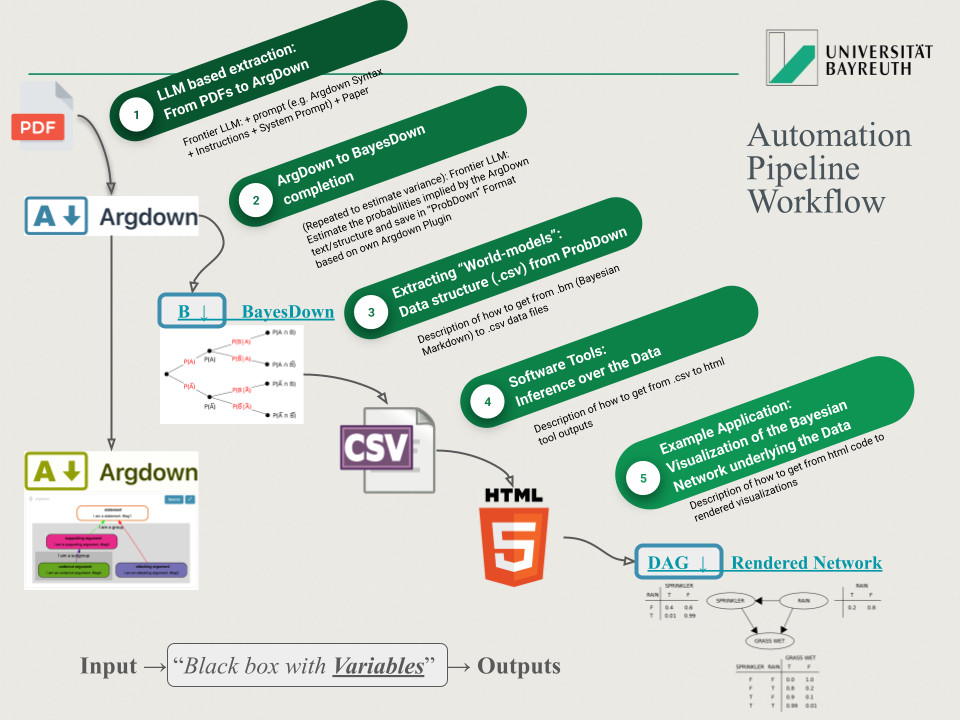
\includegraphics[width=1\linewidth,height=\textheight,keepaspectratio]{images/pipeline.png}}

}

\caption[Five-step AMTAIR automation pipeline from PDFs to Bayesian
networks]{\label{fig-automation_pipeline}AMTAIR Automation Pipeline from
\textcite{bucknall2022}}

\end{figure}%

Testing crossreferencing grapics Figure~\ref{fig-automation_pipeline}.

\begin{figure}


\includegraphics[width=0.3\linewidth,height=\textheight,keepaspectratio]{images/cover.png}

\caption[Short 2 caption]{\label{fig-testgraphic2}Caption/Title 2}

\end{figure}%

Testing crossreferencing grapics Figure~\ref{fig-testgraphic2}.

\section*{Citations}\label{sec-citations}

\markright{Citations}

\textcite{soares2014}

\autocite{soares2014} and \autocite{knuth1984}

Blah Blah \autocites[see][33-35]{knuth1984}[also][chap.~1]{growiec2024}

Blah Blah \autocite[33-35, 38-39 and passim]{knuth1984}

Blah Blah \autocite{growiec2024,knuth1984}.

Growiec says blah \autocite*{growiec2024}

\section{Headings \& Potential Headings}\label{sec-heading}

\texttt{verbatim\ code\ formatting\ for\ notes\ and\ ideas\ to\ be\ included\ (here)}

\begin{verbatim}
Also code blocks for more extensive notes and ideas to be included and checklists
- test 1. 
- test 2. 
- test 3.
2. second
3. third
\end{verbatim}

\begin{quote}
Blockquote formatting for ``Suggested Citations (e.g.~carlsmith 2024 on
\ldots)'' and/or claims which require a citation (e.g.~claim x should be
backed-up by a ciation from the literature)
\end{quote}

Here is an inline note.\footnote{Inlines notes are easier to write,
  since you don't have to pick an identifier and move down to type the
  note.}

Here is a footnote reference,\footnote{Here is the footnote.}

\renewcommand*{\labelitemi}{\textgreater}

Here's some raw inline HTML:

page 1

\newpage{}

page 2

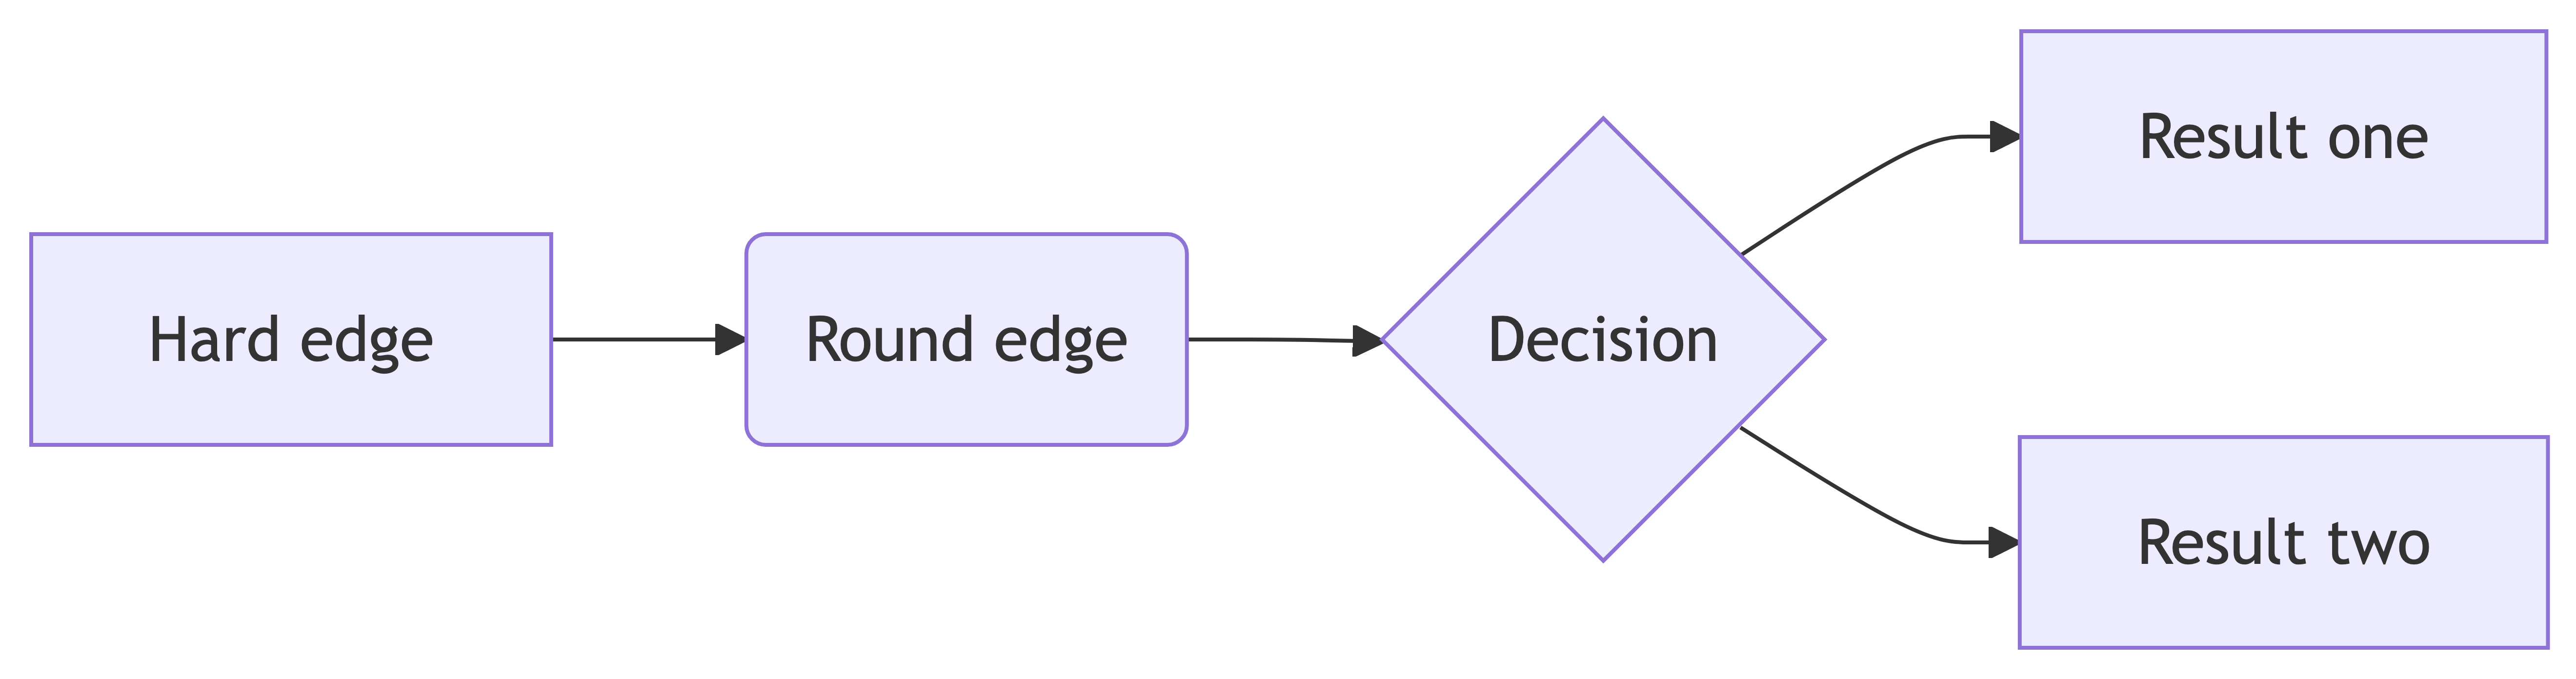
\includegraphics[width=6.88in,height=1.81in]{ref/references_files/figure-latex/mermaid-figure-1.png}

Testing crossreferencing grapics Figure~\ref{fig-automation_pipeline}.

\bookmarksetup{startatroot}

\chapter*{Bibliography (References)}\label{bibliography-references}
\addcontentsline{toc}{chapter}{Bibliography (References)}

\markboth{Bibliography (References)}{Bibliography (References)}


\cleardoublepage
\phantomsection
\addcontentsline{toc}{part}{Appendices}
\appendix

\chapter{Appendices}\label{appendices-1}

\chapter*{Appendices}\label{sec-appendices}
\addcontentsline{toc}{chapter}{Appendices}

\markboth{Appendices}{Appendices}

\section*{Appendix A: Technical Implementation
Details}\label{sec-appendix-technical}
\addcontentsline{toc}{section}{Appendix A: Technical Implementation
Details}

\markright{Appendix A: Technical Implementation Details}

\section*{Appendix B: Model Validation
Procedures}\label{sec-appendix-validation}
\addcontentsline{toc}{section}{Appendix B: Model Validation Procedures}

\markright{Appendix B: Model Validation Procedures}

\section*{Appendix C: Case Studies}\label{sec-appendix-case-studies}
\addcontentsline{toc}{section}{Appendix C: Case Studies}

\markright{Appendix C: Case Studies}

\section*{Appendix D: Ethical
Considerations}\label{sec-appendix-ethical}
\addcontentsline{toc}{section}{Appendix D: Ethical Considerations}

\markright{Appendix D: Ethical Considerations}

\chapter{appendixA}\label{appendixa}

testtext

% % Add affidavit at the end but still within document environment
% % \pagenumbering{Roman} % Switch to Roman page numbering
% 
\clearpage
\thispagestyle{empty} % Removes page numbering for current page

\newpage


% Top header with logo (left) and department (right)
\begin{minipage}{0.3\textwidth}
  
\includegraphics[width=5cm]{latex/uni-bayreuth-logo.png}
\end{minipage}
\hfill
\begin{minipage}{0.9\textwidth}
  \begin{center}
    -- P\&E Master's Programme --\\
    Chair of Philosophy, Computer\\
    Science \& Artificial Intelligence
  \end{center}
\end{minipage}

% Horizontal rule
\vspace{1.5cm}
\hrule
\vspace{2.5cm}

% Title in bold

  \LARGE\textbf{Affidavit}
\vspace{1.5cm}

\center

\normalsize

% \part*{Affidavit}

    \subsection*{\Large Declaration of Academic Honesty}
	    \vspace{1cm}\noindent \\
	    Hereby, I attest that I have composed and written the presented thesis 
        \vspace*{0.5cm}\noindent \\
        \textit{ \textbf{ Automating the Modelling of Transformative Artificial Intelligence Risks }}
        \vspace*{0.5cm}\noindent \\
        independently on my own, without the use of other than the stated aids and without any other resources than the ones indicated. All thoughts taken directly or indirectly from external sources are properly denoted as such.
	    \vspace{\baselineskip}
	    \\  This paper has neither been previously submitted in the same or a similar form to another authority nor has it been published yet.
	    \vspace{2cm}
	    
    \flushright
    \begin{minipage}{0.5\textwidth}
        \begin{flushleft} \large
        \textsc{Bayreuth}                     %   Place
        on the \\ % 26th of May 2025     \\
        \today           %   Date
        \vspace{2cm}\\
    	{\rule[-3pt]{\linewidth}{.4pt}\par\smallskip  
        \textsc{Valentin Meyer}	\\         %   Your name
    	}
        \end{flushleft}
        \end{minipage}


% \end{document}

















% % After loading packages but before \begin{document}
% \AtBeginDocument{
%   % Set up page styles
%   \fancypagestyle{frontmatter}{
%     \fancyhf{}
%     \fancyfoot[C]{\thepage}
%     \renewcommand{\footrulewidth}{0pt}
%   }

%   \fancypagestyle{mainmatter}{
%     \fancyhf{}
%     \fancyhead[LE,RO]{\slshape\nouppercase{\rightmark}}
%     \fancyhead[LO,RE]{\slshape\nouppercase{\leftmark}}
%     \fancyfoot[C]{\thepage}
%   }
% }

% % Inside the document, after title page
% \frontmatter
% \pagestyle{frontmatter}

% % Added automatically before Introduction
% % \mainmatter
% % \pagestyle{mainmatter}
